\documentclass[11pt]{article}
\usepackage{geometry}                % See geometry.pdf to learn the layout options. There are lots.
\geometry{letterpaper}                   % ... or a4paper or a5paper or ... 
%\geometry{landscape}                % Activate for for rotated page geometry
%\usepackage[parfill]{parskip}    % Activate to begin paragraphs with an empty line rather than an indent
\usepackage{graphicx}
\usepackage{amssymb}
\usepackage{amsbsy}
\usepackage{epstopdf}
\usepackage{multirow} 
\usepackage{ulem}                % So you can do \sout{ textwithstrikethroughhere }

\usepackage{sidecap}
 \usepackage{wrapfig}  % allows for wrapping text around figures
%\usepackage{url}
\usepackage{natbib}
%\usepackage{apacite}
%\usepackage{jurabib}
\usepackage[pdftex]{hyperref}
\hypersetup{
    bookmarks=true,         % show bookmarks bar?
    unicode=false,          % non-Latin characters in Acrobat�s bookmarks
    pdftoolbar=true,        % show Acrobat�s toolbar?
    pdfmenubar=true,        % show Acrobat�s menu?
    pdffitwindow=true,      % page fit to window when opened
    pdftitle={OCCAM1DCSEM: An Open-Source  Inversion Program for Generating Smooth 1D Models from Controlled-Source Electromagnetic and Magnetotelluric Data. },    % title
    pdfauthor={Kerry Key},     % author
    pdfsubject={ Electromagnetic Inversion},   % subject of the document
    pdfcreator={TexShop},   % creator of the document
    pdfproducer={}, % producer of the document
    pdfkeywords={Marine geophysics controlled source electromagetics CSEM magnetotelluric MT EM Occam inversion electrical conductivity fortran matlab}, % list of keywords
    pdfnewwindow=true,      % links in new window
    colorlinks=true,       % false: boxed links; true: colored links
    linkcolor=blue,          % color of internal links
    citecolor=blue,        % color of links to bibliography
    filecolor=magenta,      % color of file links
    urlcolor=blue           % color of external links
}

\DeclareGraphicsRule{.tif}{png}{.png}{`convert #1 `dirname #1`/`basename #1 .tif`.png}

\usepackage{url}
\urlstyle{rm}


\parindent 0in
\parskip 0pt
 
\topmargin 0in
\leftmargin -1in
\headheight 0in
\headsep 0in
\textheight 8.5in
\textwidth 6.5in
\oddsidemargin 0in
\evensidemargin 0in


%-------------------------------------------------------------------------
\begin{titlepage} 
\title{{\Huge {OCCAM1DCSEM:}} \\ \vskip0.05in
An Open-Source   Inversion Program for Generating Smooth 1D Models from Controlled-Source Electromagnetic and Magnetotelluric Data. \\  
\vskip0.45in
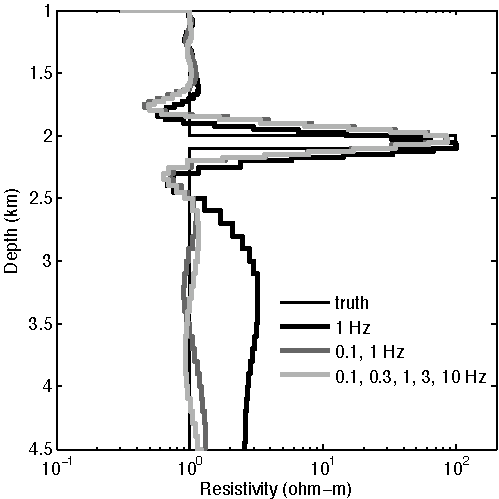
\includegraphics[]{Figures/EyFreqs.pdf} \vskip0.15in}
  
\author{  
Documentation by: \\
 Kerry Key \\
Scripps Institution of Oceanography \\
University of California, San Diego \\ \\
A product of the Seafloor Electromagnetic Methods Consortium \\
\url {http://marineemlab.ucsd.edu/semc.html} \\
\\
Revision 1.5, March 22, 2011. \\   }
\date{}                               % Activate to display a given date or no date
\end{titlepage}

%-------------------------------------------------------------------------
\begin{document}
%-------------------------------------------------------------------------
\maketitle
\newpage

%-------------------------------------------------------------------------
\tableofcontents
\newpage
\parskip 5pt
%-------------------------------------------------------------------------
%-------------------------------------------------------------------------
\listoffigures
\parskip 5pt
%-------------------------------------------------------------------------
%-------------------------------------------------------------------------
\listoftables
\newpage
\parskip 5pt
%\renewcommand{\thesection}{\roman{section}}
%




%-----------------------------------------------------------------------------------------------
\section{About}
%-----------------------------------------------------------------------------------------------
This document provides instructions for using the OCCAM1DCSEM inversion code and  the forward modeling code  DIPOLE1D.  OCCAM1DCSEM is a Fortran package for generating smooth one-dimensional  models from controlled-source electromagnetic and magnetotelluric data.   The {OCCAM1DCSEM} package is built around a new 1D CSEM forward code named DIPOLE1D, which has been designed to handle a diverse number of 1D CSEM modeling scenarios.    This package also comes with Matlab front- and rear-end routines for editing survey data, creating the files required by OCCAM1DCSEM and for plotting the resulting inversion models and CSEM responses.

 Here's a list of features currently supported in OCCAM1DCSEM and DIPOLE1D:
\begin{itemize}
\item Uses a Cartesian coordinate system, so you don't need to worry about converting to cylindrical coordinates any more
\item Models all 3 field components (x,y,z) of  both the electric and magnetic fields
\item Supports inversion of real and imaginary, amplitude and phase, and polarization ellipse data.
\item Receivers can be located anywhere in the model
\item Receiver sensor axes can be given a fixed rotation (supports full 3D rotation)
\item Option to solve for the receiver sensor orientations (supports solving for the full 3D rotation if $z$ component data available)
\item Transmitters can be located anywhere in the model
\item Transmitter antenna can be rotated both horizontally and vertically
\item Model layers are parameterized in absolute depths, not thicknesses
\item There are no assumptions of fixed layers (you have to input the air and sea layers)
\item Handles stratified seawater conductivity layering
\item Can invert for layer conductivities both above and below the receivers and transmitters.
\item Includes 1D MT inversion (alone or jointly with CSEM inversion).
\item Supports point dipoles and finite length dipoles. {\it new February 2010, thanks to David Myer for his help with this}.
\item Supports minimum gradient support roughness penalty (also known as weighted L2 regularization).  {\it new March 2010}.
\item Supports bounds on model parameters, implemented through non-linear tranforms.  {\it new March 2011}.
\end{itemize}
And here's a list of current limitations:
\begin{itemize}
\item \sout{Uses a point dipole approximation },  see above
\item Only handles isotropic conductivity
\end{itemize}
%-----------------------------------------------------------------------------------------------
\subsection{References}
%-----------------------------------------------------------------------------------------------
The forward solver Dipole1D.f90 and its application with Occam are described in: 
\begin{quotation}
\noindent
Key, K., 2009, 1D inversion of multicomponent, multifrequency marine CSEM data: Methodology and synthetic studies for resolving thin resistive layers: Geophysics, 74, F9-F20, DOI: 10.1190/1.3058434.

\end{quotation}
  
  
   The Occam's inversion algorithm is originally described in: 
   \begin{quotation}
	\noindent
       Constable, S.�C., R.�L. Parker, and C.�G. Constable, 1987, 
    Occam's inversion - A practical algorithm for generating smooth models 
    from electromagnetic sounding data: Geophysics, 52, 289-300. 
\end{quotation}
    The Orthogonal Procrustes Rotation Analysis (OPRA) method for determining the receiver orientation is 
    described in a manuscript accepted to Geophysics (January 2010):
   \begin{quotation}
	\noindent
	 Key, K. and A. Lockwood, 2010, Determining the orientation of marine CSEM 
	 receivers  using orthogonal Procrustes rotation analysis, Geophysics, 75,  F63�F70, DOI:10.1190/1.3378765.
\end{quotation}
    Please reference these papers when publishing studies conducted with this code.
    
%-----------------------------------------------------------------------------------------------
\subsection{License}
%-----------------------------------------------------------------------------------------------
  \subsubsection{Dipole1D.f90 and CSEM1D.f90 }
   
   Copyright (C) 2007-2011 \\
    Kerry Key \\
    Scripps Institution of Oceanography \\
    kkey@ucsd.edu 

    Dipole1D is free software: you can redistribute it and/or modify
    it under the terms of the GNU General Public License as published by
    the Free Software Foundation, either version 3 of the License, or
    (at your option) any later version.

    Dipole1D is distributed in the hope that it will be useful,
    but WITHOUT ANY WARRANTY; without even the implied warranty of
    MERCHANTABILITY or FITNESS FOR A PARTICULAR PURPOSE.  See the
    GNU General Public License for more details.

    You should have received a copy of the GNU General Public License
    along with Dipole1D.  If not, see \url{http://www.gnu.org/licenses/}.

   \subsubsection{Occam.f90}    
   


    Copyright (C) 1986-2011
    Steven Constable, Kerry Key, David Myer, Catherine deGroot-Hedlin
    Scripps Institution of Oceanography
    University of California, San Diego
     
    Occam's Inversion is free software: you can redistribute it and/or modify
    it under the terms of the GNU General Public License as published by
    the Free Software Foundation, either version 3 of the License, or
    (at your option) any later version.

    Occam's Inversion is distributed in the hope that it will be useful,
    but WITHOUT ANY WARRANTY; without even the implied warranty of
    MERCHANTABILITY or FITNESS FOR A PARTICULAR PURPOSE.  See the
    GNU General Public License for more details.

    You should have received a copy of the GNU General Public License
    along with Occam's Inversion.  If not, see \url{http://www.gnu.org/licenses/}.

%-------------------------------------------------------------------------
\subsection{Acknowledgments}
%-------------------------------------------------------------------------
\begin{itemize}
\item Steven Constable provided the original f77 Occam's inversion engine and gave helpful advice on incorporating the new CSEM forward solver Dipole1D.f90.
\item David Myer ported the f77 Occam code into Fortran90/95 as part of an upgrade of the Occam2DMT inversion program.  David and I have since been updating the code to Fortran2003.
\item James Gunning and John Hedditch provided helpful coding suggestions for Dipole1D.
\item David Myer initiated the modifications  to handle a finite length dipole in February 2010.
\item This work was funded by the Seafloor Electromagnetic Methods Consortium at Scripps Institution of Oceanography. See \url{http://marineemlab.ucsd.edu/semc.html} for more info. 

 The following sponsors of the Seafloor Electromagnetic Methods Consortium are thanked for their generosity:
{\small 
\begin{itemize}
\item Aker Exploration
\item Anadarko
\item  AOA Geophysics Inc
\item BG International
\item BGP International
\item BHP Billiton
\item Black Gold Energy
\item BP
\item CGG-Veritas (through 2009)
\item Chevron
\item ConocoPhillips
\item CSIRO
\item Det Norske Oljeselskap
\item Discover Petroleum (through 2009)
\item EMGS
\item ExxonMobil
\item Fugro
\item Geophysical Resources and Services
\item  GERD
\item Idemitsu Petroleum Norge AS
\item  JOGMEC
\item  Hess Corporation
\item  KMS Technologies
\item  OHM Surveys
\item  Petrobas
\item PGS
\item  Phoenix Geophysics
\item  QUASAR Federal Systems
\item  Reliance Industries
\item  Repsol YPF
\item  Rocksource ASA
\item  Santos (through 2009)
\item  Shell
\item  Statoil
\item Total
\item  WesternGeco Electromagnetics
\item  Woodside
\item  Zonge Engineering and Research Organization
\end{itemize}
}
\end{itemize}

%-------------------------------------------------------------------------
\subsection{Bugs, Fixes, Questions and Comments}
%-------------------------------------------------------------------------
Send bug reports, fixes, questions and comments to my email: \href{mailto:kkey@ucsd.edu}{kkey@ucsd.edu}.    I'll try my best to answer your questions, but don't expect an immediate reply.

%-------------------------------------------------------------------------
\section{Compiling the Source Code}
%-------------------------------------------------------------------------
For instructions on installing OCCAM1DCSEM on Unix and Windows machines, see the file "INSTALL" located in the /Source folder.  

%-------------------------------------------------------------------------
\newpage
\section{Occam's Inversion Described in a Single Page}
%-------------------------------------------------------------------------
This section is a brief overview of Occam's inversion.  It may be helpful for understanding the various parameters in the input files.   If you already have a good understanding of EM inversion, you can safely skip over to the next section. More detailed descriptions of Occam can be found in \citet{geo52-03-02890300} and \citet{geo55-12-16131624}. The specific application to marine CSEM is described in \citet{key:F9}, which is included in the /Documentation folder.

Occam's inversion seeks to minimize the following unconstrained regularized functional:
	\begin{equation}
		U = \|    \mathbf{\boldsymbol{\partial} m}   \|^{2} 
		+
		 \|    \mathbf{P( m - m_{*})}   \|^{2} 
		+ 
		\mu^{-1}\left [  \|   \mathbf{W} (\mathbf{d} - F(\mathbf{m}) )   \|^{2} - \chi_{*}^{2} \right ]  .
		\label{eq:U}
	\end{equation}
The first term is  a norm of the model roughness and is computed by applying a differencing operator $\boldsymbol{\partial}$ to the elements of the model vector $\mathbf{m}$.  For the one dimensional models considered here, $\mathbf{m}$ is a vector of  $\log_{10}\rho$ for each layer and $\boldsymbol{\partial}$ is chosen to be a matrix of first-differencing operators so that $\mathbf{\boldsymbol{\partial} m}$ approximates the vertical derivative of $\log_{10}\rho$.  The parameterization with respect to $ \log_{10} \rho$ ensures that  resistivity remains positive during the inversion. If jumps in resistivity are desired at certain depths, the corresponding elements of $\boldsymbol{\partial}$ can be set to zero.  The second term is a measure of the difference of $\mathbf{m}$ from an  a priori preference model $\mathbf{m_{*}}$. The diagonal matrix $\mathbf{P}$ contains scaling parameters that determine the relative weighting between the preference and the model roughness.   Preference model values, if used at all, are typically desired for a only few model layers and the corresponding diagonal elements of $\mathbf{P}$ will be nonzero.   The roughness and preference terms in the above equation are regularizers that serve to stabilize the inversion and keep it from producing wildly oscillating resistivity structure (see the regularized/unregularized comparisons in \citet{geo52-03-02890300}).


Finally, the third term is a measure of the misfit of the model's forward  response $F(\mathbf{m})$ (i.e., the electric and magnetic fields for model $\mathbf{m}$) to the data $\mathbf{d}$. There is no restriction on the data vector $\mathbf{d}$.  For example, it can contain data from multiple transmitters, receivers and frequencies, and can include magnetotelluric (MT) data.  $\mathbf{W}$ is a data covariance weighting function and is here selected to be a diagonal matrix with elements corresponding to inverse data standard errors.  In other words,  $\mathbf{W}$ weights the relative contribution of each datum to the misfit based on its uncertainty.  Thus, data with large errors are scaled to limit their influence, while data with small errors will have a bigger impact on the misfit budget.


 $\chi_{*}^{2}$ is the target misfit and its inclusion illustrates that minimizing $U$ does not necessarily find the best fitting model, but rather a smooth model that is within the specified target misfit.   The target misfit $\chi_{*}^{2}$ is usually chosen so that the root mean square (RMS) misfit $x_{rms}$ is equal to unity:
�\begin{equation}
	x_{rms} = \sqrt{\frac{\chi^{2}}{n} }=  \sqrt{\frac{1}{n} \sum_{i=1}^{n} \left [ \frac{d_{i}- F_{i}(\mathbf{m})}{s_{i}} \right ]^{2} },
	\label{eq:rms}
\end{equation}
where $n$ is the number of data and $s_{i}$ is the standard error of the $i$th datum.

  The Lagrange multiplier $\mu$ serves to balance the trade-off between the data fit and the model roughness and model preference.   The nonlinear minimization of equation \ref{eq:U}  is described in \citet{geo52-03-02890300} and one of the main innovations of the Occam method is the automatic selection of $\mu$.    So that's Occam described in a single page of text.  The next few sections describe the input files required to run the OCCAM1DCSEM program.

 


%-------------------------------------------------------------------------
\clearpage
\section{Model, Transmitter and Receiver Geometry}
%------------------------------------------------------------------------

The 1D model uses a right handed Cartesian geometry with the  $z$ axis pointing down, as shown in Figure \ref{fig:geometry}.   All positions are in units of meters and angles are in degrees.  There are N-layers with resistivity $\rho_{i}$  in units of ohm-m and each layer position is defined in terms of the top depth of the layer.  There are no fixed assumptions of any layer depths, including the air-sea interface.  So you will need to describe the entire model in the setup files. Receivers and transmitters can be located anywhere in the stack of layers.  When modeling real survey data, you will need to decide what the $x,y$ axes correspond to.  For example, you could use UTM coordinates and have $x=$ North, $y=$ East.  Or you could have survey local coordinates where $x=$ inline, $y=$ crossline, or $y=$ inline, $x=$ crossline.   Whatever you choose, it must be consistent between the transmitters and receivers and the angles defined below. Check and then double check that you've done the correct transformations.
\begin{figure}[htbp]
\begin{center}
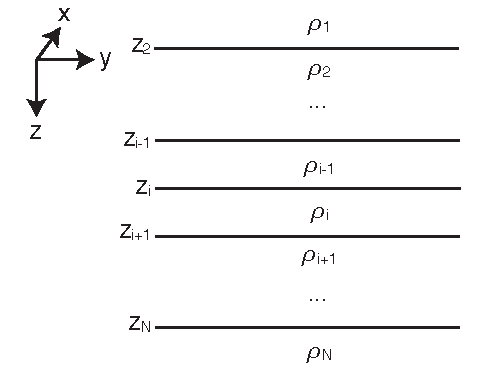
\includegraphics[width=0.72\textwidth]{Figures/nlayer.pdf}
\caption[Model geometry]{1D model geometry. There are N-layers with resistivity $\rho_{i}$ in units of ohm-m.  Each layer is defined in terms of the absolute depth of the top of the layer in units of meters.   Receivers and transmitters can be located anywhere in the stack of layers.  }
\label{fig:geometry}
\end{center}
\end{figure}
\clearpage

\subsection{Transmitter Orientation}
The transmitter orientation parameters are shown in Figure \ref{fig:TxOrient}. The transmitter azimuth  is defined to be the horizontal rotation of the transmitter antenna from the $x$ axis, positive towards $y$.  So an angle of 0 means the antenna points along $x$, while an angle of 90 degrees means the antenna points along $y$. If $x$ is also the towline direction, then the azimuth is equivalent to the antenna yaw. The transmitter dip angle is positive down from the azimuth angle. A dip of 0 degrees means the antenna is horizontal.  A dip of 90 degrees means the antenna is pointing downward.   If the tail of the antenna is sagging, the dip angle will be negative.  If the tail is higher than the head of the antenna, the dip angle will be positive.  Dipole1D supports modeling using either a point dipole approximation (faster) or a finite length dipole (slower but more accurate for short range data).  For a finite length antenna, the $(x,y,z)$ position of the antenna should be given as the antenna midpoint.  Lastly, note that the term azimuth here refers to the orientation of the antenna, not the source-receiver azimuth used in earlier cylindrical coordinate modeling parameterizations.

 \begin{figure}[htbp]
\begin{center}
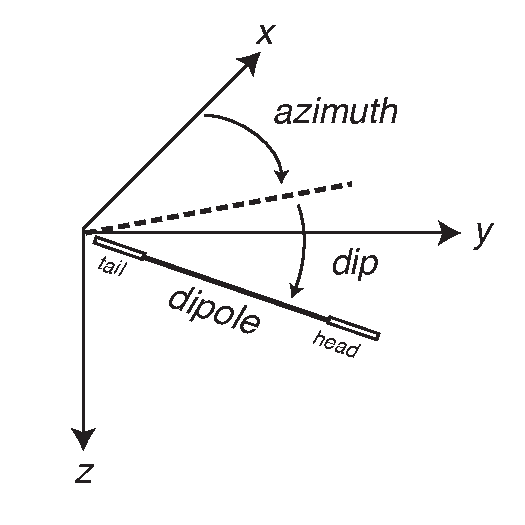
\includegraphics[width=0.49\textwidth]{Figures/TxOrient}
\caption[Transmitter orientation parameters]{  Transmitter orientation parameters.  The transmitter azimuth is defined to be the horizontal rotation of the transmitter antenna from the $x$ axis, positive towards $y$.  So an azimuth of 0 means the antenna points along $x$, while an angle of 90 degrees means the antenna points along $y$. The transmitter dip angle is positive down from the azimuth angle.  }
\label{fig:TxOrient}
\end{center}
\end{figure}

 
\clearpage
\subsection{Receiver Orientation \label{sec:ReceiverOrient}}
  OCCAM1DCSEM can model receiver data pre-rotated to the survey axes $(x,y,z)$, or at whatever arbitrarily rotated axes the data are collected along $(x'',y'',z'')$.  To do this, the full 3D rotation of the receiver needs to be specified using three angles.  The orientation of the sensor axes  $(x'',y'',z'')$  from the survey axes $(x,y,z)$ can be described by three angles: $\theta, \alpha$, and $\beta$, as shown in Figure \ref{fig:RxRotParams}. Below I give a mathematical description of these rotation parameters.
  
%\begin{wrapfigure}{r}{0.55\textwidth}
\begin{figure}
\begin{center}
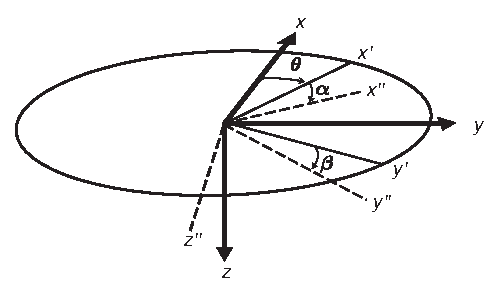
\includegraphics[width=.75\textwidth]{Figures/3DRotationAxes.pdf}
\caption[Receiver orientation parameters]{ Rotation parameters for the absolute orientation of  receiver sensors along axes $(x'',y'',z'')$.  Rotation in the horizontal plane can be described by the angle $\theta$, which is the rotation about the $z$ axis from the survey axes $(x,y)$ into $(x',y')$.  The tilt of the receiver can be specified with the angles   $\alpha$ and $\beta$, which describe rotations about the $y'$ and $x''$ axes, respectively.  Note that $\alpha$ describes tilt in a vertically oriented plane along $\theta$, while the angle $\beta$ describes tilt along a dipping plane when $\alpha\ne 0$. The circle denotes the horizontal plane.}
\label{fig:RxRotParams}
\end{center}
\end{figure}



The complex valued  vector electric and magnetic field data $\mathbf{F}''$ recorded in the receiver's rotated  coordinate system  are  related to the  fields $\mathbf{F}$ in the survey coordinate system by a $3 \times 3$ orthonormal rotation matrix $\mathbf{R}$ as
	\begin{equation}
	\mathbf{F}'' =  \mathbf{F}\mathbf{R}.
	\label{eq:Rotation}
	\end{equation}
  For $n$ discrete source-receiver offsets, $\mathbf{F}$ and $\mathbf{F}''$ can be written as $2n \times 3$ arrays:
	\begin{equation}
	\mathbf{F} =
		\left[
		\begin{array}{ccc}
		 \mathrm{Re}(F_{x,1}) & \mathrm{Re}(F_{y,1})& \mathrm{Re}(F_{z,1}) \\
		  \mathrm{Im}(F_{x,1}) &  \mathrm{Im}(F_{y,1})& \mathrm{Im}(F_{z,1}) \\
		 \vdots  & \vdots  & \vdots \\
		 \mathrm{Re}(F_{x,n}) & \mathrm{Re}(F_{y,n})& \mathrm{Re}(F_{z,n}) \\
		  \mathrm{Im}(F_{x,n}) &  \mathrm{Im}(F_{y,n})& \mathrm{Im}(F_{z,n}) \\
		\end{array}	 
		\right],
	\end{equation}
where $F_{x,i}$ specifies the $x$ component of the $i$-th datum and the real and imaginary parts of the complex data have been separated into alternating rows.	  The rotation matrix $\mathbf{R}$ can be written as a product of rotations about individual axes:
	 \begin{equation}
		\mathbf{R} = \mathbf{R}_{z}\mathbf{R}_{y'}\mathbf{R}_{x''},
	\end{equation}
where
	\begin{equation}
	\mathbf{R}_{z} =
		\left[
		\begin{array}{rrr}
		\cos({\theta}) & -\sin({\theta}) & 0 \\
		\sin({\theta}) & \cos({\theta})  & 0  \\
		0 & 0  & 1  \\
		\end{array}	 
		\right],
	\end{equation}
	\begin{equation}
	\mathbf{R}_{y'} =
		\left[
		\begin{array}{rrr}
		\cos({\alpha}) & 0 & -\sin({\alpha})  \\
	          0 & 1 & 0 \\
		\sin({\alpha}) & 0 & \cos({\alpha})   \\
		\end{array}	 
		\right],
	\end{equation}
and
	\begin{equation}
	\mathbf{R}_{x''} =
		\left[
		\begin{array}{rrr}
		 1 & 0 & 0 \\
		0 &\cos({\beta}) & -\sin({\beta})  \\
		0 & \sin({\beta}) & \cos({\beta})   \\
		\end{array}	 
		\right].
	\end{equation}
$\mathbf{R}_{z}$ is a rotation by $\theta$ about the $z$ axis, giving new coordinate axes ($x',y',z$). $\mathbf{R}_{y'}$ is a rotation by $\alpha$ about the $y'$ axis, giving new coordinate axes ($x'',y',z'$). $\mathbf{R}_{x''}$ is a rotation by $\beta$ about the $x''$ axis, giving the final rotated axes ($x'',y'',z''$). 

If you specify non-zero rotation parameters for a given receiver, then OCCAM1DCSEM will rotate the model response to the data orientation using equation \ref{eq:Rotation}.


%-------------------------------------------------------------------------
\clearpage
\section{Input Files Required by OCCAM1DCSEM}
%------------------------------------------------------------------------
OCCAM1DCSEM requires three input files: IterationFile, ModelFile, and DataFile.    These files are simple text files and use a flexible format that  allows for blank lines and comments (text after ! and \% signs is ignored).  The basic structure for many of the lines in these files is {\it keyword : value}, where {\it keyword} specifies a parameter to set and {\it value} is the value to use. They are separated by a colon.  All text fields  are case insensitive, except for the strings listing file names.  Certain {\it keyword : value} pairs are followed with arrays of numbers (receiver or transmitter locations, etc). Also, don't be a moron and  use file names that have spaces in them :)

 The following subsections describe the details of each file, and you can also study the examples provided with the OCCAM1DCSEM code distribution in the folder /Examples.  Additionally, there is a Matlab routine called createEMDataFile.m which you can use to convert data to the correct format and to create the IterationFile, ModelFile, and DataFile.  So if you tire easily when reading verbose file format descriptions, skip on ahead to the Matlab code section and remember to refer back to this section if you have any problems.

\newpage
%-------------------------------------------------------------------------
\subsection{Iteration File Format \label{sec:IterFile}}
%-------------------------------------------------------------------------
The IterationFile is the first file read by OCCAM1DCSEM and specifies the parameters that Occam's inversion will use to begin its search for the smoothest model that fits the data.  By default, this file is named ``startup'' on the first iteration of Occam, but a different file name can be specified using a command line argument (described in Section \ref{RunOcc}).  The code is backwards compatible with the older format OCCAMITER\_1.0, but I strongly recommend using David Myer's new flexible format  OCCAMITER\_FLEX.    Here is an example IterationFile, with brief descriptions after the ! symbol:

{\footnotesize 
\begin{verbatim}
Format:             OCCAMITER_FLEX      ! Flexible format
Description:        test                ! Not used by Occam, but you can use this for your own notes.
Model File:         model               ! Name of the Model File. Case sensitive.
Data File:          data                ! Name of the Data File. Case sensitive.                                                                      
Date/Time:          11/25/2008 16:46:39 ! On output, date and time stamp placed here.          
Max Iter:           100                 ! Maximum number of Occam iterations to compute.
Target Misfit:      1.0                 ! Target RMS misfit, see equation 2.
Roughness Type:     1                   ! See section below for Roughness Penalty options
!Model Bounds:      min,max             ! Optional, places bounds on log10(rho) values.
!Model Value Steps: stepsize            ! Optional, forces model into discrete steps of stepsize.
Debug Level:        1                   ! Console output. 0: minimal, 1: default, 2: detailed
Iteration:          0                   ! Iteration number, use 0 for starting from scratch.
Lagrange Value:     5.000000            ! log10(largrance multiplier), starting value.
Roughness Value:    0.1000000E+08       ! Roughness of last model, ignored on startup
Misfit Value:       100.0000            ! Misfit of model listed below. Ignored on startup
Misfit Reached:     0	                  ! 0: not reached, 1: reached.  Useful when restarting.
Param Count:        75                  ! Number of free inversion parameters.
     0             ! A listing of the free inversion parameter values in log10(resistivity).    
     0             ! Here the 0's correspond to log10(1 ohm-m).
     0             ! Since this is iteration 0, the inversion will thus be started with a 
     0             ! 1 ohm-m halfspace.
     0
     0
     0
     0
     0
     0
     0
     0
...
\end{verbatim}
}
Note that the Model Bounds and Model Value Steps fields are optional. If you want to use these, then remove the ! comments at the beginning of the lines.

%-------------------------------------------------------------------------
\subsubsection{Roughness Type Options }
%-------------------------------------------------------------------------
Occam1DCSEM supports a few options for the roughness penalty used to regularize (i.e., stabilize) the non-linear inversion.     The roughness type parameter can either be entered as an integer code or as a string value, as listed in Table \ref{tab:RougnessCodes}.
\begin{table}[htdp]
\caption{Roughness Type Options }
\begin{center}
{
\begin{tabular}{lll}
Integer Code & String Code & Description \\
\hline
 1 & `FirstDiff' &  First differencing penalty, {\it default value}\\
 4 & `DepthWeighted' &  log10(depth) weighted penalty \\
   & `mgs, $\delta$' &  Minimum gradient support penalty \\
\end{tabular}
}
\end{center}
\label{tab:RougnessCodes}
\end{table}%

The roughness penalty corresponds to the term $ \|    \mathbf{\boldsymbol{\partial} m}   \|^{2} $ in equation \ref{eq:U}, but here we generalize this into the roughness operator $\mathcal{R}$:
\begin{equation}
\|   \mathcal{R}(\mathbf{m})  \|^{2}  =  \|  \mathbf{W_\mathcal{R}}  \mathbf{\boldsymbol{\partial} m}   \|^{2} ,
\end{equation}
where $\mathbf{W_\mathcal{R}} $ is a diagonal weighting matrix that varies according to the roughness penalty type.  For standard first differencing, $\mathbf{W_\mathcal{R}} =\mathbf{I}$, meaning the weights are all unity. This is the default regularization used by Occam1DCSEM. 

For  Depth Weighted roughness, the  diagonal elements of $\mathbf{W_\mathcal{R}}$ are the logarithm of the depth  of each layer (relative to the top layer).  In other words, the roughness penalty slowly increases with depth in the model.    

For minimum gradient support, the weight values have a more complicated form that depends on the gradient of the previous model's conductivity parameters. If the current model parameter vector is $\mathbf{m}_{j+1}$, then the {\it i}-th diagonal element of $\mathbf{W_\mathcal{R}}$ has the form
\begin{equation}
\mathbf{W}_{\mathcal{R}}(i)  = \frac{1} { \sqrt{  (\mathbf{m}_j(i) - \mathbf{m}_j(i-1))^2 + \delta^2  }}
\end{equation}

This form of the weighting allows for a relaxation of the roughness penalty in regions where the model begins to develop {\it large} gradients in the model parameters.  The definition of {\it large} is controlled through the $ \delta$ parameter, which also keeps the denominator from going to zero.  This type of roughness penalty is also known as weighted L2 regularization.  For further discussion, see   
\citet{portniaguine:874} and \citet{vanDenBerg2001}.    To use minimum gradient support, set the roughness type using:

{\footnotesize 
\begin{verbatim}
Roughness Type:     mgs,0.1                 
\end{verbatim}
}
where 0.1 or another desired value specifies $\delta$.

Examples of the effect of the various roughness operators are shown in Figure \ref{fig:MGS} at the end of these instructions.  In our experience, the standard first differencing roughness operator is the most reliable for keeping the inversion process stable so that it can find a model at the target RMS.  The minimum gradient support roughness penalty allows for much sharper features to develop, often producing a more geologically satisfying model.  However, this regularization is much less stable; it is not uncommon for the inversion can get stuck in local minima before it obtains the target RMS (this of course also depends on the assigned value of $\delta$).    For example, standard first differencing might be able to fit a data set to RMS 1.0, whereas the minimum gradient support roughness might result in the inversion getting stuck at RMS 2.1 or something else much larger than 1.0.  If this happens, trying inverting with different values for $\delta$ until the inversion is able to fit the data as well as the standard first difference  roughness penalty (if at all).

%-------------------------------------------------------------------------
\subsubsection{Bounding the model parameters (New March 2011) }
%-------------------------------------------------------------------------
Suppose you have good reason(s) to bound the model parameters, such that $ b < m < a$, where $b$ and $a$ are lower and upper bounds.  This can be done in Occam using a nonlinear transformation of the model parameters from $m$ to function $x(m)$, where the inverse transform $m(x)$  is bound by $ b < m(x) < a$.  With this framework, the inversion no longer inverts for $m$, but rather inverts for the unbound parameter $x$. However, since $m(x)$ is bound, the inversion can no longer generate model parameters outside the bounds since  for large positive $x$, $m(x)$ is asymptotes to $a$, while at large negative $x$, $m(x)$ asymptotes to $b$.        Occam1DCSEM supports two different transform methods. The exponential transform has seen recent use for EM inversion \citep{Habashy:2004ux,Commer:2008gb}:
\begin{eqnarray}
m(x) &=& \frac{a e^x +b }{e^x + 1} \;\;\;\;\;\mathrm{where}   \;\;\;\;\;\; b < m < a
\end{eqnarray}
This transform has a peak in its sensitivity transform $\partial m / \partial x$ and the transformed parameters can look quite different than the original parameters, even inside the bounds. That inspired me to try building a transform that has a sensitivity transform that looks like a band pass filter, with a flat response between the bounds.  After a bit of tedious manipulations with a simple bandpass filter formula, I found the `bandpass' transform to be
\begin{eqnarray}
m(x) &=& \frac{ac + \log \left (\frac{ 1+ e^{c(b-x)}}{1+e^{c( a-x)}} \right )}{c (1-e^{-c(a-b)})}   \;\;\;\;\;\mathrm{where}   \;\;\;\;\;\; b < m < a \\
 && \mathrm{and}\;\;\;\; c = {15}/(a-b)
\end{eqnarray}
A visual benefit of the bandpass transform is that inside the bounds, the parameters are the same as the original parameters, see Figure \ref{fig:mcomp} for a comparison.
\begin{figure}[htbp]
\begin{center}
\includegraphics[]{Figures/mcomp.pdf} 
\caption{Comparison of the exponential transform (red) with the bandpass transform (blue).   }
\label{fig:mcomp}
\end{center}
\end{figure} 
In my own inversion tests, both of these transforms seem to work well and I have yet to find one to be consistently better than the other.

The choice of transform and the specific model bounds can be specified in the iteration file using:
{\footnotesize 
\begin{verbatim}
Bounds transform:   bandpass          
Model Bounds:       0,3       ! <lower>,<upper>
\end{verbatim}
}
or for the exponential transform:
{\footnotesize 
\begin{verbatim}
Bounds transform:   exponential   
Model Bounds:       0,3           
\end{verbatim}
}
The default transform is `bandpass' and in that case you just need to specify the bounds.
In these examples the model parameters are bound between 0 and 3 (ie., $10^0 - 10^3$ ohm-m).  See Figure \ref{fig:Bounds}  for an example of using the bounds to improve the inversion result.


%-------------------------------------------------------------------------
\newpage
\subsection{Model File Format}
%-------------------------------------------------------------------------
The model file describes the 1D model layering and denotes whether a given layer has a fixed resistivity or is a free inversion parameter.  It also specifies the roughness penalty weight applied across each layer boundary, and whether any free layers have preferred resistivity values.      Note that while the Iteration file uses log10(resistivity) for the inversion parameters, the model file uses linear resistivity for any fixed layers or any preference layers (see below).  Here is an example model file using the only currently supported format,  Resistivity1DMod\_1.0:

{\footnotesize
\begin{verbatim}
Format: Resistivity1DMod_1.0
#Layers:    77
! Layer block listing is:  
! [top_depth 	resistivity    penalty	 preference   pref_penalty] 
      -100000       1d12           0           0           0  ! Air, fixed layer of 10^12 ohm-m
           0         0.3           0           0           0  ! Sea, fixed layer of 0.3 ohm-m
        1000          -1           1           0           0  ! First free layer, the seafloor @ 1000 m 
        1025          -1           1           0           0  ! use -1 or ? to denote free layer resistivity
        1050          -1           1           0           0
        1075          -1           1           0           0
        1100          -1           1           0           0
        1125          -1           1           0           0
        1150          -1           1           0           0
        1175          -1           1           0           0
        1200          -1           1           0           0
        1225          -1           1           0           0
        1250          -1           1           0           0
        1275          -1           1           0           0
        ...
\end{verbatim}
        }
The layer top depth is given in absolute units as meters and the top depth of the first layer is ignored by Dipole1D.  Fixed resistivities are given in units of \textbf{linear} resistivity (ohm-m).  For example, the above example has two fixed layers, the air (1d12 ohm-m, or $10^{12}$ ohm-m) and a single sea layer (0.3 ohm-m).  However, you could also include a stratified seawater resistivity profile, as described in \citet{key:F9}.  

 For free inversion layers, the resistivity value is flagged as a free parameter using either of a -1 or a ?.  The penalty value is an user specified  weight applied the roughness operator, as applied to the resistivity jump across each layer boundary where both layers resistivities are free parameters.   Usually this will just be a 1.  If you want to allow a jump in conductivity at a certain depth, you can relax the roughness penalty at that depth by setting the penalty weight to 0 (or something smaller than 1) at that layer boundary depth.   Here's an example matrix representation of how the penalty weights ($w_{i}$) are applied to the default first difference roughness operator (matrix of 1's and -1's) and the model vector ($m_{i}$) in equation \ref{eq:U}, for a simplistic 5 layer model:
\begin{eqnarray*}
\mathbf{\boldsymbol{\partial} m} &=&\left[\begin{array}{rrrrr}w_1 & 0 & 0 & 0 & 0 \\0 & w_2 & 0 & 0 & 0 \\0 & 0 & w_3 & 0 & 0 \\0 & 0 & 0 & w_4 & 0 \\0 & 0 & 0 & 0 & w_5\end{array}\right]\left[\begin{array}{rrrrr}0 & 0 & 0 & 0 & 0 \\-1 & 1 & 0 & 0 & 0 \\0 & -1 & 1 & 0 & 0 \\0 & 0 & -1 & 1 & 0 \\0 & 0 & 0 & -1 & 1\end{array}\right]
\left[\begin{array}{c}m_1 \\m_2 \\m_3 \\m_4 \\m_{5}\end{array}\right]
\end{eqnarray*}
The form of the weights is flexible.  Usually just a 1 is sufficient. However, you could make the penalty weights ($w_{i}$) increase with depth if you thought there was a good geological reason for the model to be smoother with depth.  Or you could scale them by the layer thicknesses if you want the roughness penalty to approximate  the vertical spatial derivative.

 The preference value is the  \textbf{linear} resistivity (ohm-m) that you might prefer for certain layers, although this feature is not commonly used.   For example, you might have a priori geologic information that a certain layer is probably resistive, and you can impart this preference on Occam by specifying the preferred value. A good case for using a preference value is when you want to test a hypothesis of whether a certain layer is resistive (or conversely conductive).  You can invert the data with the preference value given and see how well Occam is able to fit the data.  If the inversion isn't able to fit the data well, or the inverted resistivity is far from the preference, you might be able to rule out the presence of certain structures.    Also, in some inversions i've performed on real survey data, i've found that adding penalty cuts to the roughness operator can sometimes destabilize the inversion to the point of it wandering off to infinity.  I was able to re-stablize the inversion by setting some preference resistivity values for the thin layers between the penalty jumps.  However, beware that adding too many cuts and preference resistivity values will ultimately turn a fairly objective inversion into a ``desired output" filter.

 
 
  If you want a preference value, then you need to also set the pref\_penalty (its weight) to a non-zero value (1 is the nominal value), otherwise it will be ignored when pref\_penalty=0.  Here's a matrix representation of the preference terms in equation \ref{eq:U} for a simplistic 5 layer model:
\begin{eqnarray*}
  \mathbf{P( m - m_{*})}&=&\left[\begin{array}{rrrrr}p_1 & 0 & 0 & 0 & 0 \\0 & p_2 & 0 & 0 & 0 \\0 & 0 & p_3 & 0 & 0 \\0 & 0 & 0 & p_4 & 0 \\0 & 0 & 0 & 0 & p_5\end{array}\right]
\left[\begin{array}{c}m_1 - m_{*1} \\m_2 - m_{*2} \\m_3 - m_{*3} \\m_4 - m_{*4} \\m_5 - m_{*5}\end{array}\right]
\end{eqnarray*}
So setting the preference penalty  weight  $p_{i}>0$ and preference resistivity $m_{*i}$ means that the difference in  $m_i - m_{*i}$ will be minimized by the inversion, subject to the constraint that the data still needs to be fit.  Note that the preference value is given as linear resistivity, but internally this is converted to log10(resistivity).  
Here's a toy example ModelFile that includes two cuts in the roughness penalty, a preferred resistivity layer and uses ? instead of -1 to denote the free parameter layers: 

{\footnotesize
\begin{verbatim}
Format: Resistivity1DMod_1.0
#Layers:    77
! Layer block listing is:  
! [top_depth 	resistivity    penalty	 preference   pref_penalty] 
      -100000       1d12           0           0           0  ! Air, fixed layer of 10^12 ohm-m
           0         0.3           0           0           0  ! Sea, fixed layer of 0.3 ohm-m
        1000           ?           1           0           0  ! First free layer, the seafloor @ 1000 m 
        1025           ?           1           0           0  ! use -1 or ? to denote free layer resistivity
        1050           ?           1           0           0
        1075           ?           1           0           0
        1100           ?           0           0           0  ! Allows a resistivity jump at 1100 m
        1125           ?           1           0           0
        1150           ?           0           0           0  ! Allows a resistivity jump at 1150 m
        1175           ?           1           0           0
        1200           ?           1          55           1  ! A 55 ohm-m preferred layer, spanning 
        1225           ?           1          55           1  ! from  1200-1250 m depth
        1250           ?           1           0           0
        1275           ?           1           0           0
        ...
\end{verbatim}
        }
%-------------------------------------------------------------------------
\newpage
\subsection{Data File Format}
%-------------------------------------------------------------------------

The data file lists the transmitters, receivers and frequencies, and has a table of data parameters, values and standard errors.  The currently supported data formats are  named  EMData\_1.1 and EMData\_1.2 (technically EMData\_1.0 is still supported, but it was lacking so I won't describe it here).  This format is designed to be compatible with future 2D and 3D inversion codes and hence is very general.  Like the Iteration and Model files, the Data file format can include arbitrary comment lines (using ! or \%) or blank lines.  Here's an example DataFile:
\begin{verbatim}
Format:  EMData_1.2
Dipole Length: 250        ! [m] Optional, the default is 0 m which is a point dipole
# integ pts:   10         ! Optional and only used if Dipole Length > 0. 
# Transmitters:   41
!          X            Y            Z      AZIMUTH          DIP
           0            0          950           90            0   
           0          500          950           90            0 
           0         1000          950           90            0 
          ...
# Frequencies:    2
         0.1
           1
# Receivers:      20
!           X          Y            Z         Theta        Alpha         Beta
            0          0         1000             0            0            0 
            0       1000         1000             0            0            0     
            0       2000         1000             0            0            0 
           ...                           
# Data:       714
!         TYPE        FREQ#        TX#            RX#       DATA 	  SD_ERROR
        RealEy            1            1            1 -2.94217e-07  5.86785e-09 
        ImagEy            1            1            1  4.71955e-10  5.86785e-09 
        RealEz            1            1            1  6.95924e-09  5.86785e-09 
        ImagEz            1            1            1 -1.35431e-09  5.86785e-09 
        RealBx            1            1            1  2.89886e-11  5.84098e-13 
        ImagBx            1            1            1 -1.82912e-13  5.84098e-13 
        RealEy            1            2            1  5.35934e-10  1.08866e-11 
        ImagEy            1            2            1  7.50943e-11  1.08866e-11 
        RealEz            1            2            1 -4.89381e-11  1.08866e-11 
          ...
\end{verbatim}
 
The Transmitters block lists the transmitter dipole length, the number of transmitters and then the $x,y,z$ (meters) locations of the transmitters, and their rotation angle (degrees clockwise from x) and dip angle (degrees positive down).   Note that both the ``Dipole Length" parameter is optional.  Set this to a non-zero positive number to model a finite length dipole.  The parameter ``\# integ pts" is optional and is only used if  ``Dipole Length" $> 0$.  This parameter specifies the number of points to use to the Gauss quadrature integration for the finite length dipole.  A default value of 10 is used if you don't specify a value in the data file.  The runtime of the code increases with this parameter (each integration point is an additional transmitter to model), so you may want to optimize this parameter for your particular data set.  For example, you might be able to get away with a value of 2 or 3 if you are at least a couple of dipole lengths away from the transmitter. 

The Frequencies block lists the number of frequencies and then the values (Hz).

The Receivers block lists the number of receivers and then the $x,y,z$ (meters) positions of the receivers and each receiver's rotation angles, as shown in Figure \ref{fig:RxRotParams}.

The Data block lists the number of data and  then contains a table of data parameters, data and standard errors.  The first column of the data table specifies the data type.  The currently supported data types for CSEM and MT data are given in Table \ref{tab:DataCodes}.   The data type can be specified using either the string codes or the numeric codes given in Table \ref{tab:DataCodes}.  The string values are not case sensitive.  The second column of the data table is the frequency index for each datum. The third column is the transmitter index and the fourth column gives the receiver index.  The fifth and sixth columns are the data and standard errors. Electric fields should be given in units of V/Am$^{2}$ and magnetic fields in units of T/Am.  For MT data, the impedances are in units of ohms, apparent resistivities in units of linear ohm-m and phases in degrees.  Impedance phases (for Zyx) should be moved to the first quadrant (nominally 45 degrees, not -135 degrees).


\begin{table}[htdp]
\caption{Data types used in format EMData\_1.1}
\begin{center}
{\footnotesize
\begin{tabular}{llll}
& Integer Code & String Code & Description \\
\hline
CSEM Data: &1 & RealEx & Real Ex \\
 &2 & ImagEx & Imaginary Ex\\
 &3 & RealEy & Real Ey\\
 &4 & ImagEy  & Imaginary Ey\\
 &5 & RealEz & Real Ez\\
 &6 & ImagEz & Imaginary Ez\\
\\
 &11 & RealBx & Real Bx\\
 &12 & ImagBx & Imaginary Bx\\
 &13 & RealBy & Real By\\
 &14 & ImagBy & Imaginary By\\
 &15 & RealBz & Real Bz\\
 &16 & ImagBz & Imaginary Bz\\
\\

 &21 & AmpEx & Amplitude Ex\\
 &22 & PhsEx & Phase Ex \\
 &23 & AmpEy & Amplitude Ey\\
 &24 & PhsEy & Phase Ey \\
 &25 & AmpEz & Amplitude Ez\\
 &26 & PhsEz & Phase Ez \\
\\
 &31 & AmpBx & Amplitude Bx\\
 &32 & PhsBx & Phase Bx \\
 &33 & AmpBy & Amplitude By\\
 &34 & PhsBy & Phase By \\
 &35 & AmpBz & Amplitude Bz\\
 &36 & PhsBz & Phase Bz \\
\\ 
&41 & PEmax & Electric horizontal polarization ellipse maximum \\
&42 & PEmin  & Electric horizontal polarization ellipse minimum\\
&43 & PBmax &Magnetic  horizontal polarization ellipse maximum\\
&44 & PBmin  & Magnetic  horizontal polarization ellipse minimum\\
\\
MT Data: 
 &101 & RhoZxx & Apparent Resistivity Zxx, ignored in 1D \\
 &102 & PhsZxx & Phase Zxx, ignored in 1D\\
 &103 & RhoZxy & Apparent Resistivity Zxy \\
 &104 & PhsZxy & Phase Zxy \\
 &105 &RhoZyx & Apparent Resistivity Zyx \\
 &106 & PhsZyx & Phase Zyx \\
 &107 & RhoZyy & Apparent Resistivity Zyy, ignored in 1D\\
 &108 & PhsZyy & Phase Zyy, ignored in 1D\\
\\
 &111 & RealZxx & Real Zxx, ignored in 1D \\
 &112 & ImagZxx & Imaginary Zxx, ignored in 1D\\
 &113 & RealZxy & Real Zxy \\
 &114 & ImagZxy & Imaginary Zxy \\
 &115 & RealZyx & Real Zyx \\
 &116 & ImagZyx & Imaginary Zyx \\
 &117 & RealZyy & Real Zyy, ignored in 1D\\
 &118 & ImagZyy & Imaginary Zyy, ignored in 1D\\
\end{tabular}
}
\end{center}
\label{tab:DataCodes}
\end{table}%

That covers the basics of the data file.  However, there are a few optional fields that may help you deal with the details of real survey data.  These are explained in the following sections.  These are not required in the Data file, but if present they are used.
\clearpage
%-----------------------------------------------------------------------------------------------
\subsubsection{Phase Convention \label{sec:Phase} }
%-----------------------------------------------------------------------------------------------
The default convention used in DIPOLE1D is phase lag (i.e., phases become increasingly positive with source-receiver offset), but you can instead specify that the data use a phase lead convention (i.e., phases become increasingly negative with source-receiver offset):
{\small
\begin{verbatim}
Phase Convention: lag         ! Optional, use lag (default) or lead 
 \end{verbatim}  
 }

%-----------------------------------------------------------------------------------------------
\subsubsection{Solving For Unknown Receiver Rotations \label{sec:OPRA} }
%-----------------------------------------------------------------------------------------------
There is an option for specifying that the receiver rotations are unknown and then the inversion will solve
for the best fitting rotations.  Simply put, you just list ? for the receiver angles instead of numeric values.   Here's how it works.

The geometry of the receiver orientation was described in section \ref{sec:ReceiverOrient}.  The receiver's rotation angles shown in Figure \ref{fig:RxRotParams} can be estimated by solving  the minimization problem:
	 \begin{equation}
	\min _{\mathbf{R}} \; \|  \hat \mathbf{F}'' - \hat\mathbf{F}\mathbf{R} \|_F^{2} \; \; \mathrm{subject\; to} \; \; \mathbf{R}^{{T}}\mathbf{R} = \mathbf{I},
	\label{eq:MinProb}
	\end{equation}
where $\mathbf{I}$ is the identity matrix and  the Frobenius norm $\|\mathbf{ A} \|_F^{2} =\mathrm{tr}(\mathbf{A}^T\mathbf{A})$.  The data arrays are normalized using   $\hat \mathbf{F}''  = \mathbf{W} \mathbf{F}''$ and $\hat \mathbf{F}  = \mathbf{W} \mathbf{F}$, where the  weighting function $\mathbf{W}$ is a diagonal matrix of  the inverse data standard errors  that serves to reduce the contribution of noisy data.  Although we can never know the true unrotated field vector  $\mathbf{F}$, we can approximate it using the forward response from each Occam iteration.  The minimization of the above equation is then accomplished using the Orthogonal Procrustes Rotation Analysis (OPRA) method \citep{key:F63}.
 
 This is available as an option for  OCCAM1DCSEM inversions. To use the OPRA method, you will need to set the receiver orientation angles to ? marks:
 
\begin{verbatim}
...
# Receivers:      1
!           X          Y            Z         Theta        Alpha         Beta
            0          0         1000             ?            ?            ? 
           ...                           
\end{verbatim}
Most of the time there will be only a single receiver (as shown above).  However, you could solve for multiple receiver orientations or have some combination of known and unknown receivers all in the same data file.

There are some restrictions on the data array if you enable the OPRA method.  First, the data must be given as real/imaginary components and they must be listed by site in order as RealEx, ImagEx, RealEy, ImagEy, RealEz, ImagEz, etc, as shown in this example below.  Also note that the data standard errors must be isotropic among all $x,y,z$ components. Typically I use some fraction (1-10\%) of the total vector amplitude as the standard error.
\newpage
\begin{verbatim}
!         TYPE        FREQ#        TX#           RX#       DATA 	  SD_ERROR
           1            1            1            1  2.04917e-07  5.86785e-09 
           2            1            1            1  2.49658e-09  5.86785e-09 
           3            1            1            1  2.20625e-07  5.86785e-09 
           4            1            1            1  -3.7858e-10  5.86785e-09 
           5            1            1            1  1.71885e-08  5.86785e-09 
           6            1            1            1 -2.68835e-09  5.86785e-09 
           1            1            2            1 -3.80006e-10  1.08866e-11 
           2            1            2            1 -5.97309e-11  1.08866e-11 
...
\end{verbatim}

You can also include magnetic field data using the same ordering.  If the data only contains the horizontal components, then only the angle $\theta$ will be estimated. If the data contain all $x,y,z$ components then all three angles $\theta,\alpha,\beta$ will be estimated.

OCCAM will then find the best orientation angles during each inversion iteration and  these are written out to a file with the name ``iter\_X.rotations'', where X is the iteration number.  The model response files (.resp) will have the data and model responses rotated to the cartesian $x,y,z$ axes, and this is noted in the ``Receiver Orientations'' block of the response file.  So in other words, the data in the data file will be in the original receiver orientation while the data and responses in the .resp file are aligned along $x,y,z$.

Some synthetic rotated data examples are given in   the /Canonical\_Solve\_3DRotation and /Canonical\_Solve\_HorizRotation folders in the /Examples folder.  See the comments in the data files there for what the data orientation angles are.  For both of these examples, OCCAM1DCSEM and OPRA are able to fit the data to RMS 1.0 and find the orientations angles to about  $1^{\circ}$ error.  For real data with 2D and 3D structures, you might find reasonable orientation estimates by using either short offset data (dominated by diffusion through the seawater), or by using only long offset data (dominated by diffusion through air), but this depends on how non-1D the structure is and on how reliably the transmitter and receiver positions are known.
 


\clearpage
%-----------------------------------------------------------------------------------------------
\subsubsection{A Note about 1D Reciprocity}
The bulk of the inversion CPU time is dominated by the 1D CSEM forward and sensitivity computations.  These computations depend linearly on the number of discrete transmitter locations.  Thus, the fewer the transmitters, the faster the runtime. For 1D modeling, it is often possible to use reciprocity to convert multiple transmitters into multiple receivers, and hence speed up the runtime. If you input a vector of transmitters
that all have the same depth, azimuth and  dip but different x,y positions, the code is smart enough to apply 1D reciprocity and convert the transmitters into many receivers and will then run much faster.   This is all done automatically and as an end user you should only notice that the runtime is fast.  Conversely, if the input transmitters are depth varying or have varying dips and azimuths then 1D reciprocity is not used and the runtime can be substantially longer.   There are some additional ways to speed up the code for varying dips and azimuths, but I haven't code them up yet since for the most part the code should run fast enough for most users needs.


%-----------------------------------------------------------------------------------------------
\subsubsection{A Note about Standard Errors}
This section contains some notes that might be useful for converting the data uncertainties between real and imaginary components and amplitude and phase.  The complex CSEM data $z$ can be represented in either form by using Euler's formula:
\begin{equation}
z = r e^{i \phi} = u + i\, v,
\end{equation}
where $r$ is the amplitude, $\phi$ is the phase, $u$ is the real component,  $v$ is the imaginary component and $i = \sqrt{-1}
$.  These are shown graphically in Figure  \ref{fig:Errors}.
We generally assume that the data uncertainty $\delta z$ is isotropic with respect to the complex data $z$, as shown by the gray circle in the figure.  This is written as
\begin{equation}
\delta z= \delta u + i \,\delta v,\;\;\; \mathrm{where}\;\;\;\delta u = \delta v.
\end{equation}
Isotropic uncertainty  also means the amplitude uncertainty $\delta r = \delta u = \delta v$.   Lastly, the uncertainty in the phase $\phi$ can be found by noting that the arc length associated with isotropic uncertainty $\delta r$ is
\begin{equation}
r \delta \phi \approx \delta r.
\end{equation}
Therefore, the corresponding phase uncertainty $\delta \phi$ is
\begin{equation}
\delta \phi \approx  \frac{\delta r}{r} \frac{180}{\pi},
\end{equation}
where the last factor converts radians to degrees.  For example, a relative uncertainty ${\delta r / r} = 1\% $ has a corresponding phase uncertainty $\delta \phi = 0.573^{\circ}$ , while ${\delta r / r} = 10\% $ gives $\delta \phi = 5.73^{\circ}$.   

\begin{figure}
\begin{center}
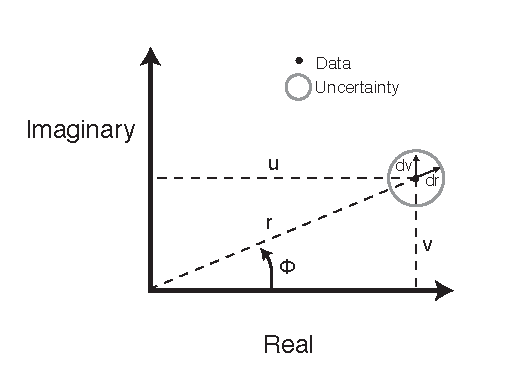
\includegraphics[width=.75\textwidth]{Figures/Errors.pdf}
\caption[Complex data and uncertainty diagram]{ Complex data and uncertainty diagram showing the relationship between real and imaginary components ($u$ and $v$) and amplitude ($r$) and phase ($\phi$). }
\label{fig:Errors}
\end{center}
\end{figure}
\clearpage


%-------------------------------------------------------------------------
\newpage
\section{Running OCCAM1DCSEM \label{RunOcc}}
%-------------------------------------------------------------------------
Thanks to David Myer's efforts, Occam now supports a few command line parameters for specifying run options.
To run OCCAM1DCSEM, use this syntax:
\begin{verbatim}
OCCAM1DCSEM [-F] [ <IterationFileName> [<OutputFileNameRoot>] ]
\end{verbatim}
where all the quantities inside [ ] are optional. \\
\\
Options:
\begin{description}
\item[-F ]  Specifies to compute only the forward response of the starting IterationFile.  The response is written out to a .resp file.
\item[IterationFileName ]  Specifies the IterationFile to start Occam with.  If this file is not given, then Occam by default will assume that the name of the starting IterationFile is ``startup''.
\item[OutputFileNameRoot ]  Specifies the root name for all files output during the Occam inversion.
\end{description}

Here are a few examples:

\begin{verbatim}
$ OCCAM1DCSEM
\end{verbatim}
Here Occam will read in the file ``startup'' and each iteration, model response and Occam logfile will be output to the files iter\_X.iter and iter\_X.resp and and logfile.logfile, where X is the iteration number.
\begin{verbatim}
$ OCCAM1DCSEM Trough.iter Trough
\end{verbatim}
Here Occam will read in the file ``Trough.iter '' and each iteration, model response and Occam logfile will be output to the file Trough\_X.iter and Trough\_X.resp and and Trough.logfile.
\begin{verbatim}
$ OCCAM1DCSEM Trough_20.iter Trough
\end{verbatim}
Here Occam will begin with the iteration file ``Trough\_20.iter ''  which is presumeably the 20th iteration of a previous Occam run.
\begin{verbatim}
$ OCCAM1DCSEM -F  MyHypothesisModel
\end{verbatim}
Here Occam reads in the startup file ``MyHypothesisModel''  and will compute the forward response and misfit of  MyHypothesisModel, and will then output the response to the file ``MyHypothesisModel.resp''.

When OCCAM1DCSEM begins, it will print out the information contained in the Data and Model files and will then proceed with the Occam iterations.  During each iteration, the misfit as a function of Lagrange multiplier and model roughness will be output to the terminal console.  At the end of each iteration, the best model misfit, roughness and Lagrange multiplier values are output to the console. Much of this information is also written to the .logfile.


%-------------------------------------------------------------------------
\newpage
\subsection{Output Files}
%-------------------------------------------------------------------------
At the end of each iteration Occam will output an IterationFile with the best model parameters found during that iteration.  This file has the same format as the input IterationFile described in Section \ref{sec:IterFile}.  Additionally, the response of those model parameters is written out to a .resp file.   The .resp file is nearly the same as the data file, but the data table portion is a \#data $\times$ 8 array expanded to include the model response. The first six columns are
just a copy of the data parameters, data and standard errors given in the data table, the seventh and  eighth columns are the model response and the normalized residual (i.e., the number of standard deviations for the fit of that datum):
�\begin{equation}
 \mathrm{residual} = \frac{d_{i}- F_{i}(\mathbf{m})}{s_{i}} 
	\label{eq:residual}
\end{equation}
Here's an example of the data/response section of the response file:

{\footnotesize 
\begin{verbatim}
! Type      Freq#          Tx#          Rx#          Data      StdError      Response      Residual
   3            1            1            1  -0.29857E-06   0.58679E-08  -0.29039E-06         -1.39
   4            1            1            1  -0.10099E-08   0.58679E-08   0.49898E-09         -0.26
   5            1            1            1  -0.23965E-08   0.58679E-08   0.54621E-08         -1.34
   6            1            1            1  -0.50163E-08   0.58679E-08   0.44280E-11         -0.86
  11            1            1            1   0.29732E-10   0.58410E-12   0.29506E-10          0.39
  12            1            1            1   0.54974E-12   0.58410E-12   0.10734E-12          0.76
   3            1            2            1   0.52793E-09   0.10887E-10   0.53702E-09         -0.84
   4            1            2            1   0.82776E-10   0.10887E-10   0.80643E-10          0.20
   5            1            2            1  -0.32813E-10   0.10887E-10  -0.29366E-10         -0.32
   6            1            2            1   0.17868E-10   0.10887E-10   0.86575E-11          0.85
          ...
\end{verbatim}
}
\clearpage                   
%-----------------------------------------------------------------------------------------------
\newpage
\section{DIPOLE1D - 1D Forward Modeling}
%-----------------------------------------------------------------------------------------------
The Fortran program DIPOLE1D can be used for rapid forward model studies.  
DIPOLE1D requires a single input file name RUNFILE to compute CSEM responses. 
See the folder Dipole1D located provided with several of the test data sets in /Examples/Synthetic for an example RUNFILEs.   The .csem response files output by DIPOLE1D can be plotted using plotCSEM.m and you can also use them to create synthetic noisy data files with the createEMDataFile.m user interface.  If you're only interested in computing forward responses for various models, DIPOLE1D is much simpler to setup than using Occam with the -F command line option (which requires that you also build the data table).        


%-----------------------------------------------------------------------------------------------
\subsection{Calling DIPOLE1D directly from Matlab}
%-----------------------------------------------------------------------------------------------
In addition to running DIPOLE1D in a terminal window, you can now call it
directly from Matlab, thanks to David Myer's efforts at writing the requisite
 Mex file for DIPOLE1D.  To get this working on you system, see read the 
 instructions in the file INSTALL.txt  in /Source.  Here's the Matlab help text for
 running mexDipole1D.m:
  
 \begin{verbatim}
  ! MatLab interface for Kerry Key's Dipole1D CSEM forward model code.
  ! Gateway function code patterned after 'yprimefg.f' MatLab example code.
  !
  ! David Myer
  ! Copyright 2009
  ! Scripps Institution of Oceanography
  ! dmyer@ucsd.edu
  !
  ! This function ('mexDipole1D' in MatLab, NOT 'MEXFUNCTION') definition:
  ! Params:
  !       nTransmitter - array with cols: X, Y, Z, Azimuth, Dip
  !       nFreq        - vector of frequencies
  !       nLayers      - array with cols: TopDepth, Resistivity
  !       nReceiver    - array with cols: X, Y, Z
  !       nTalk        - (optional) 0=say nothing, 1=show fwd calls, 
  !                       2=spew lots of text (default)
  !       bPhaseConv   - (optional) 0=phase lag (dflt), 1=phase lead
  !       nDipoleLen   - (optional; dflt=0) length of dipole in meters centered
  !                       at the transmitter position(s).  0 = point dipole.
  !       numIntegPts - (optional; dflt=10) number of integration points
  !                       for Gauss quadrature integrations for finite dipole computations.
  !
  ! Returns:
  !       nFields     - array with cols: 
  !                       Xmtr #, Freq #, Rcvr #, Ex, Ey, Ez, Bx, By, Bz
  !                     Sorted by columns 1,2,3
\end{verbatim}
%-----------------------------------------------------------------------------------------------
\newpage
\section{Matlab  Editing and Plotting Tools}
%-----------------------------------------------------------------------------------------------
There are a few Matlab plotting routines in the /Matlab directory for editing data, and plotting up the inversion models, the data and the model responses.     To use these, you will need to add this directory and its subdirectories to Matlab's search path.  You can do this in Matlab by selecting ``File $\rightarrow $ Set Path...'', then clicking the ``Add with subfolders'' button and then selecting the /Matlab directory.  These routines should meet most users' plotting needs.  If you want to use your own custom plotting routines, you might find the file reading kernels in the directory  /Matlab/a\_utils useful.

Here's  a summary of the routines, and the next few sections describe the details for each:
\begin{table}[htdp]
\begin{center}
\begin{tabular}{lp{4in}}
createEMDataFile.m & An interactive graphical user interface for editing data  and creating the data, model and startup files used by {OCCAM1DCSEM}. \\
plotCSEM.m & An interactive GUI for plotting data and model responses. \\
plotOccam1DCSEM.m & Plots the inversion models. \\
plotOccam1DCSEMIterMisfit.m & Plots the search performance of the Occam inversion iterations.
\end{tabular}
\end{center}
\end{table}



The data plotting routines currently support these data file formats:
\begin{table}[htdp]
\begin{center}
\begin{tabular}{lp{4in}}
EMData\_1.1, EMData\_1.2 & Occam1DCSEM data file format \\
EMResp\_1.1, EMResp\_1.2 & Occam1DCSEM  model response file format \\
Dipole1D\_1.0, Dipole1D\_1.1 & DIPOLE1D forward model response file format \\
MARE2DCSEM\_2.0 & MARE2DCSEM finite element forward modeling code response file format. 
\end{tabular}
\end{center}
\label{tab:plotCSEMformats}
\end{table}

***If you would like to have your data format supported, kindly send me a description of the format and an example file and I'd be happy to add code to support it.  Or you can do this yourself by looking at the code readCSEM.m in the /Matlab/plotCSEM/a\_util folder and adding a call to a function that reads your data format into the CSEM structure defined in readCSEM.m.


%-----------------------------------------------------------------------------------------------
\newpage
\subsection{Editing EM Data files with createEMDataFile.m}
%-----------------------------------------------------------------------------------------------
This utility is a graphical user interface that reads in CSEM data and allows you to select which components and frequencies to output, set rotations, set noise levels, select good and bad data segments, and will then output an EMData\_1.1 format data file.  It can also be used to create the model and startup files required by OCCAM1DCSEM.  You can also use this tool to read in forward model responses compute by MARE2DCSEM or DIPOLE1D, add noise to them and then create a synthetic data file for inverting with OCCAM1DCSEM.  

  The createEMDataFile.m user interface is called by typing this into the Matlab command window:
\begin{verbatim}
  >> createEMDataFile
\end{verbatim}
The user interface shown in Figure \ref{fig:createEMDataFile} will then appear.

\begin{figure}[htbp]
\begin{center}
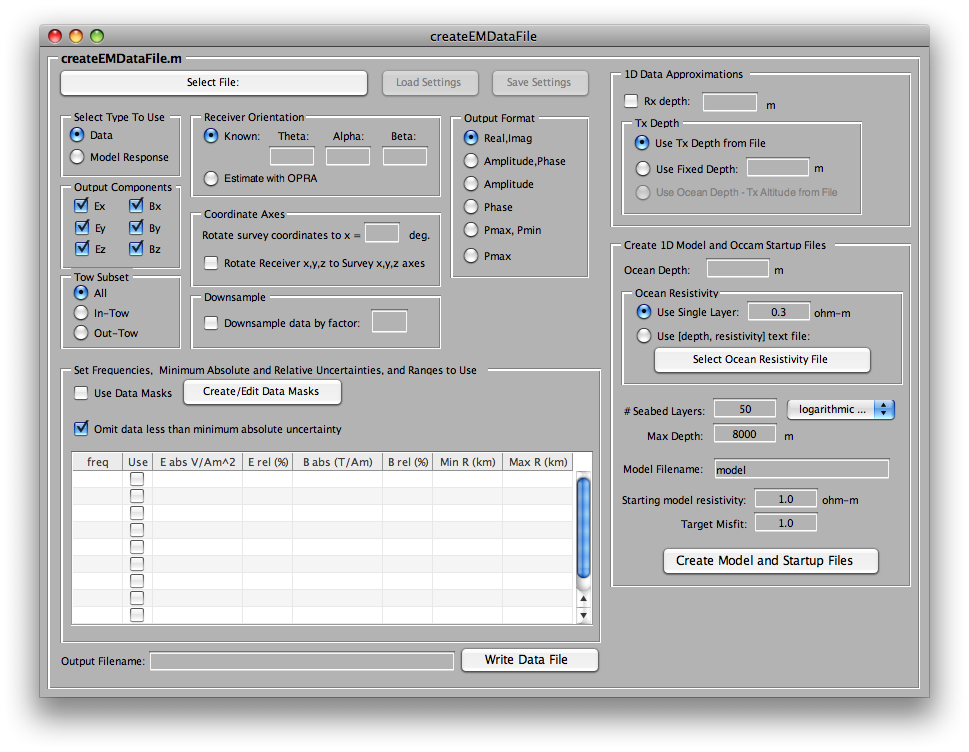
\includegraphics[width=\textwidth]{Figures/createEMDataFile}
\caption[createEMDataFile.m Matlab  interface]{The Matlab interface for createEMDataFile.m. }
\label{fig:createEMDataFile}
\end{center}
\end{figure}
\clearpage

Below are  some instructions on what the various buttons do, listed by panel starting in the top left of the user interface. 

\subsubsection*{Select File}
 Select a CSEM data file for editing.  Note that createEMDataFile.m currently only supports single site data, so if you give it a file with more than one receiver, it will ask you to select which receiver to use.
 
 \subsubsection*{Select Type To Use}
 Allows you to select which data type to output.  Normally you don't need to do anything and will just use the default value Data.  However, if you want to do synthetic inversions of forward model responses, then select the Model Response option.  For this case, the model responses will have random normally distributed noise added to them (according to the relative levels specified in the Uncertainty table) before they are written to the output Data File.

 \subsubsection*{Output Components}
 Select which components to output.  Note that the x,y,z channels are relative to the instrument reference frame, which is not necessarily the same as the survey reference frame.
 
  \subsubsection*{Tow Subset}
  This option allows you to output only a subset of the CSEM tow, either all data or only the in-tow or out-tow data.
  
   \subsubsection*{Receiver Orientation}
   This option allows you to specify the orientation of the receiver using the three angles shown in Figure \ref{fig:RxRotParams}.   Or you can select the Estimate with OPRA button if you want to use the orientation estimation method described in section \ref{sec:OPRA} .  Note that if you select OPRA, then all  components of the data will be automatically selected for output, and the Output Format will be automatically selected as Real,Imag.  If you don't want either of the E's or B's to be used with OPRA, then deselect them.  Just make sure that you include all x,y (and possibly z) components of whatever fields you're using with the OPRA method.
   
    \subsubsection*{Coordinate Axes}
    You can enter an angle to rotate the horizontal survey coordinate axes to (defined clockwise from x towards y).  Or just leave it blank to skip any rotation of the survey axes.   You can also select the Rotate Receiver checkbox if you want the receiver to be rotated so that its x,y,z channels are aligned with the survey x,y,z channels (this option is disabled if OPRA selected).
    
     \subsubsection*{Downsample}
If you have lots of data the inversion can take a long time to run.  Often you may want a quick inversion run while you're investigating the noise levels and other features of the data.  This option allows you to only output every nth data point.  For example if you enter the number 5 in this box, only data from every 5th transmitter position will be output in the data file.  Leave this blank to not downsample the data.  Note that this does not stack nor average the data.

     \subsubsection*{Output Format}
 This option allows you to select the output format for the data as one of Real and Imaginary, Amplitude and Phase, Amplitude only, Phase only,  Polarization ellipse Maximum and Minimum  (in the horizontal plane) or, Polarization Maximum only.
     
        \subsubsection*{Set Frequencies, Minimum Absolute and Relative Uncertainties, and Ranges to Use}
        
        \subsubsection*{Use Data Masks}  Select this option to use a mask file to denote good and bad data.  Click the Create/Edit Data Masks button to launch an interactive tool for selecting the good and bad data by pointing and clicking in plot of the CSEM response for each frequency.  Figure \ref{fig:DataMask} shows an example of the data mask edit figure.  The figure shows the electric and magnetic field responses for a given frequency.  Deselected data is shown in gray and will not be included in the output data file, while selected data is shown in color.  Buttons along the top of the figure allow you to select or deselect  data, or to move on to the next frequency. Click on  Select All and Deselect All buttons to select or deselect all data in a given plot.  After hitting one of these, just click in inside either of the electric or magnetic field plots to select or deselect all data for that field (note that this work simultaneously on both the amplitude and phases, regardless of which axes you click inside).  The Select+ and Deselect- buttons allow you to select discrete positions of data to omit, based on the position of the transmitter.  After hitting one of these buttons click once to select the left or right side of the selected region, then click again on the right or left side of the selected region and then the selected/deselected data on the plot will be updated.  Hit the Next or Previous buttons to scroll through the available frequencies in the data file.        When you're done selecting data, hit the Quit and Save button.  The mask file is then saved to $<$filename$>$.masks, where $<$filename$>$ is replaced with the name of the data file.  Note that when you click on Create/Edit data masks, the code looks for this file and will load it in and use it if it exists. 
        
     
  \begin{figure}[h]
\begin{center}
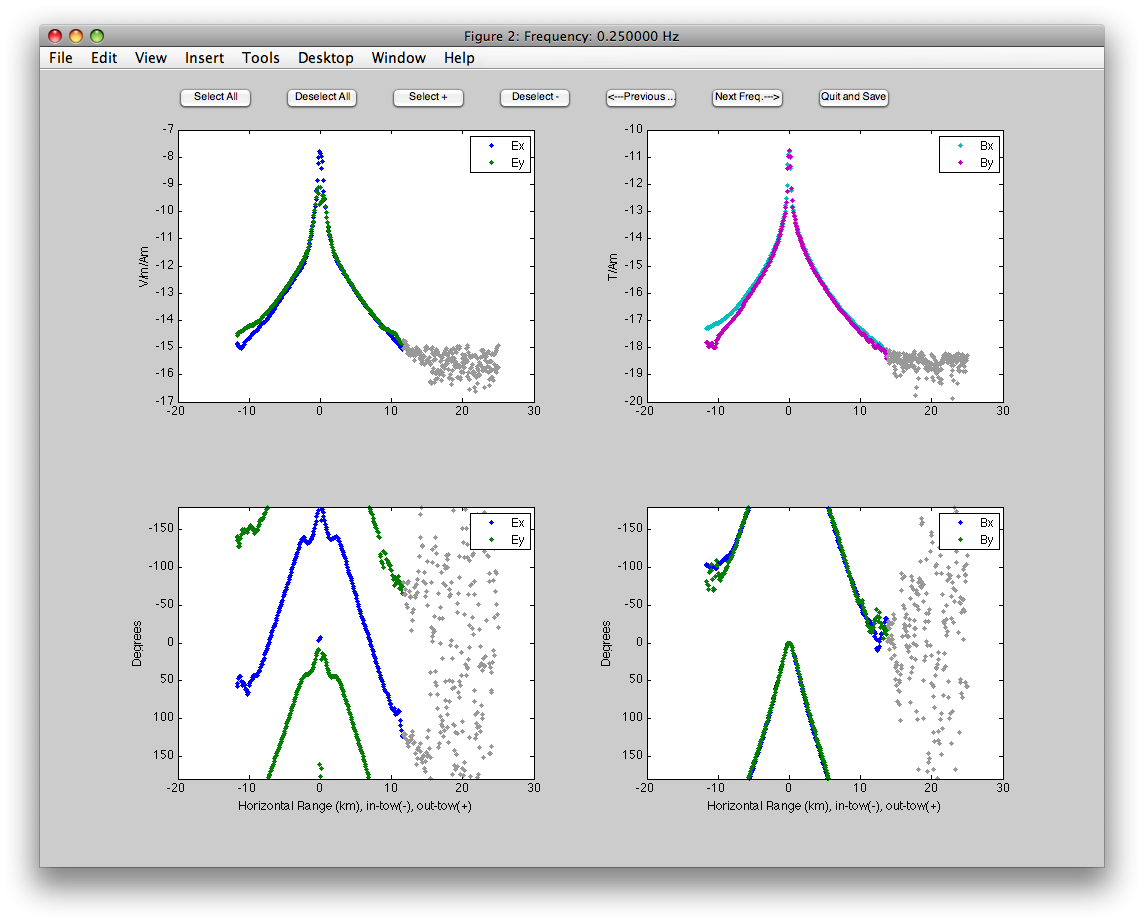
\includegraphics[width=\textwidth]{Figures/DataMask}
\caption[Create/Edit Data Mask Figure Example.]{Create/Edit Data Mask Figure Example.}
\label{fig:DataMask}
\end{center}
\end{figure}
\clearpage       

        \subsubsection*{Omit data less than minimum uncertainty}
        This option will omit data with amplitudes smaller than those given in the Uncertainty table.
        
         \subsubsection*{Uncertainty table}
         This table allows you to select the frequencies to output, to set the minimum relative and absolute noise levels for each field and to set limits on the minimum and maximum source-receiver ranges to use.   You can enter in values for each frequency, or if you want the same values for each frequency, just enter some numbers in the first row (as shown in Figure \ref{fig:UncertaintyTable}) and the code will use this for all the frequencies.
         
    \begin{figure}[h]
\begin{center}
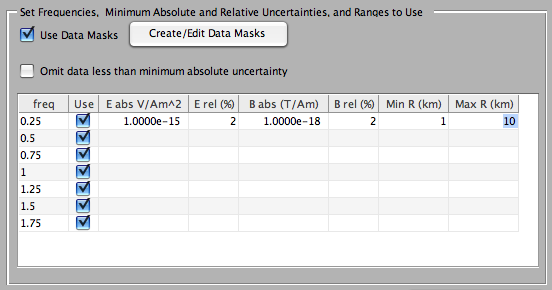
\includegraphics[width=.7\textwidth]{Figures/UncertaintyTable}
\caption[Uncertainty Table.]{The Uncertainty table allows you to select frequencies, set noise levels and range bounds on the output data.}
\label{fig:UncertaintyTable}
\end{center}
\end{figure}
\clearpage                     
                
                
         \subsubsection*{Output Filename}
         Allows you to specify the name of the output data file.  By default this is set to $<$filename$>$.emdata, $<$filename$>$ is  the name of the data file you selected at the start.  If you want a different name, just change it here.  
         
           \subsubsection*{Write Data File}    
           Hit this button and the code writes out the data file using all the parameters you've specific in the user interface.  A little message box will pop up letting you know its done outputting the file.  If you have a big data file, this can take a few seconds.
           
           \subsubsection*{1D Data Approximations}
           This panel allows you to set some parameters that are useful for 1D modeling approximations.  For example, you may want to change the transmitter and receiver depths from the values given in the original data file when the survey line has lots of topography (which isn't modeled in 1D). 
           
               \subsubsection*{Receiver Depth}
               By default the receiver depth in the original data file is displayed, but you could change it here if you need to.
               
             \subsubsection*{Transmitter Depth} 
             If you're going to do 2D/3D modeling with bathymetry, then you probably want the Use Tx Depth from File button selected.  For 1D modeling, you will need to select a Fixed Depth to use (so that the transmitter depth doesn't go below the 1D seafloor when the survey line has lots of regional slope!).    I'm planning on having another option here that might be useful for 1D approximations (Use Ocean Depth - Tx Altitude), but the altitude measurements i've seen in the raw data files can be quite unreliable at times, and so this option is disabled for now.  
                
                \subsubsection*{Create 1D Model and Occam Startup Files}   
                This panel has parameters that allow you to create the Model and Startup files easily.
                
        \subsubsection*{Ocean Depth}                  
                Enter the depth of the ocean.  By default this is set to be the same as the Rx depth, but you could change it if you have a towed receiver or a borehole receiver.
                
                \subsubsection*{Ocean Resistivity}
                You can enter a single value for a uniform seawater layer, but you'll probably be better off using CTD or XBT data to use a more accurate stratified seawater resistivity (mainly from thermal layering). Use the Select Ocean Resistivity File button to read in a two column file of [ depth (m), resistivity (ohm-m)] for the seawater.     
                
          \subsubsection*{\# Seabed Layers}
          Number of model layers to use for the seafloor.  The popup menu allows you to select  uniform or logarithmically increasing layer thicknesses.  I usually use around 20-100 layers and set a maximum depth of less than  8 km.  
          
              \subsubsection*{Max Depth}
              Maximum depth of the seabed layering (m).
              
                  \subsubsection*{Model Filename}
                  Name of the model file.  Default is ``model''.
                  
            \subsubsection*{Starting model resistivity}           
            The resistivity value for starting Occam with a uniform halfspace.  Use units of linear ohm-m and the code will do the log10 conversion for you.
            
            \subsubsection*{Target misfit}
            The target misfit for Occam.  
            
            \subsubsection*{Create Model and Startup Files}
            Hit this button to write out the Model and Startup Files.  If you done this and written the data file, then you're ready to run OCCAM1DCSEM.
                            

%-----------------------------------------------------------------------------------------------
\newpage
\subsection{Plotting inversion models with plotOccam1DCSEM.m }
%-----------------------------------------------------------------------------------------------
plotOccam1DCSEM.m is a Matlab code for plotting the inversion models output by OCCAM1DCSEM.
Make sure you change Matlab's Current Directory to the directory where you ran the inversion. 
Then use one of these commands:
\begin{verbatim}
   >> plotOccam1DCSEM   % asks you to select the iteration file to plot
 
   >> plotOccam1DCSEM('MyIterationFile.iter') % plots MyIterationFile.iter
 
   >> plotOccam1DCSEM('lastiter') % plots the most recent iteration in the
                                    current directory
 
   >> plotOccam1DCSEM('alliter') % plots all iterations in the current
                                   directory
 
   >> plotOccam1DCSEM({myiters}) % plots all iteration files in the cell
                                   array 'myiters'

\end{verbatim}
Figure \ref{fig:plotOccam1DCSEM} shows some example plots made with plotOccam1DCSEM.m.  If you don't like repeatedly typing this rather lengthy name into the Matlab command line, I recommend that you set this command as a shortcut button on the Matlab tool bar.
                                  
\begin{figure}[htbp]
\begin{center}
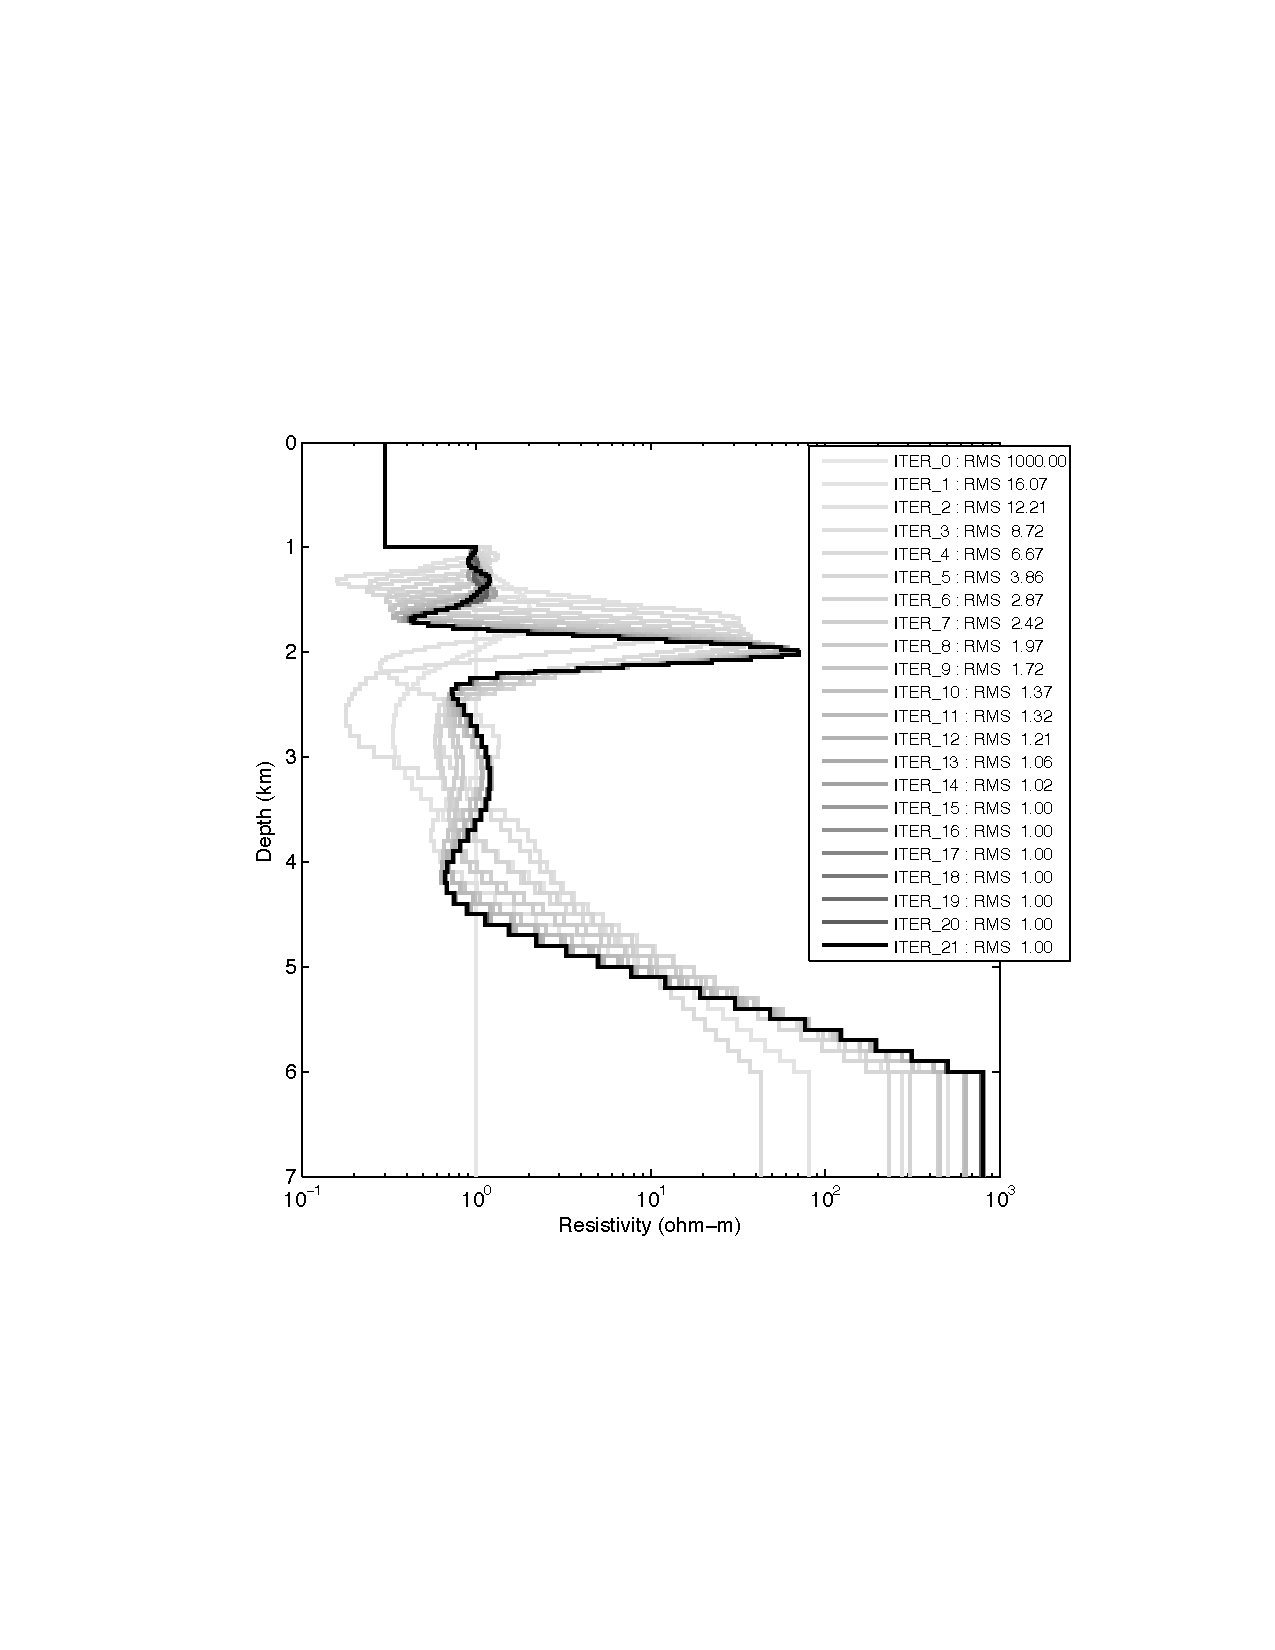
\includegraphics[width=.48\textwidth]{Figures/AllIter.pdf}
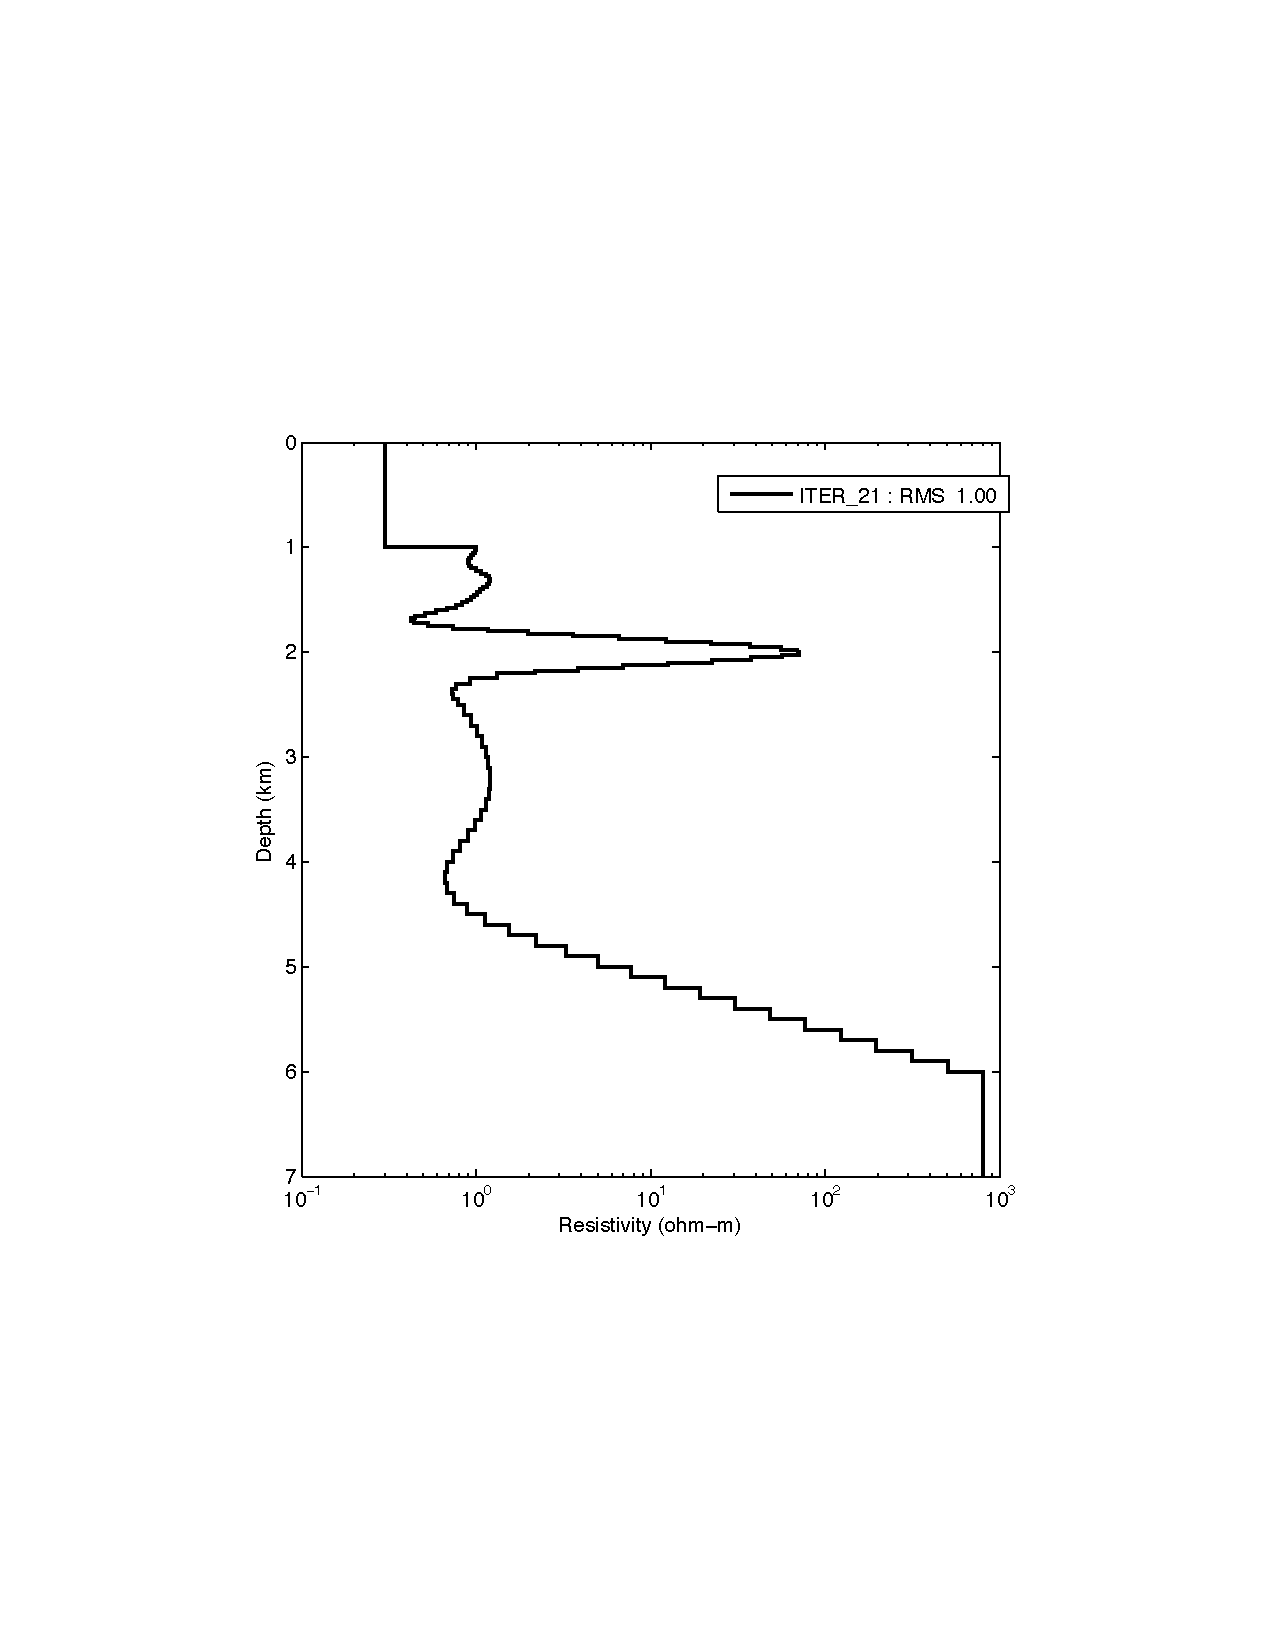
\includegraphics[width=.45\textwidth]{Figures/Iter21Single.pdf}
\caption[plotOccam1DCSEM.m examples]{ plotOccam1DCSEM.m examples.  The figure on the left is generated using ``plotOccam1DCSEM('alliter') ''  and shows the 21 iterations for that inversion.  The iterations are colored in grayscale with the highest (and presumably best) iteration plotted in black. The figure on the right is generated using  ``plotOccam1DCSEM('lastiter')'' or ``plotOccam1DCSEM('ITER\_21.iter')'' and just contains the inversion model for a single iteration.}
\label{fig:plotOccam1DCSEM}
\end{center}
\end{figure}
\clearpage
                              
                                  
\subsection{Plotting the behavior of Occam's inversion with plotOccam1DCSEMIterMisfit }
This command plots up parameters that describe the search performance of the Occam inversion iterations.  This routine will probably not be used much, but it is useful if the inversion fails or for studying the rare case where it seems unstable. \\ \\
Usage:
\begin{verbatim}
>> plotOccam1DCSEMIterMisfit  % reads in all iteration  files in the current 
% directory and plots misfit and roughness versus iteration, also
% plots search data recorded in the .logfile.  
\end{verbatim}
Figure \ref{fig:plotOccamIterMisfit} shows two example plots made with plotOccam1DCSEMIterMisfit.m.  

  \begin{figure}[htbp]
\begin{center}
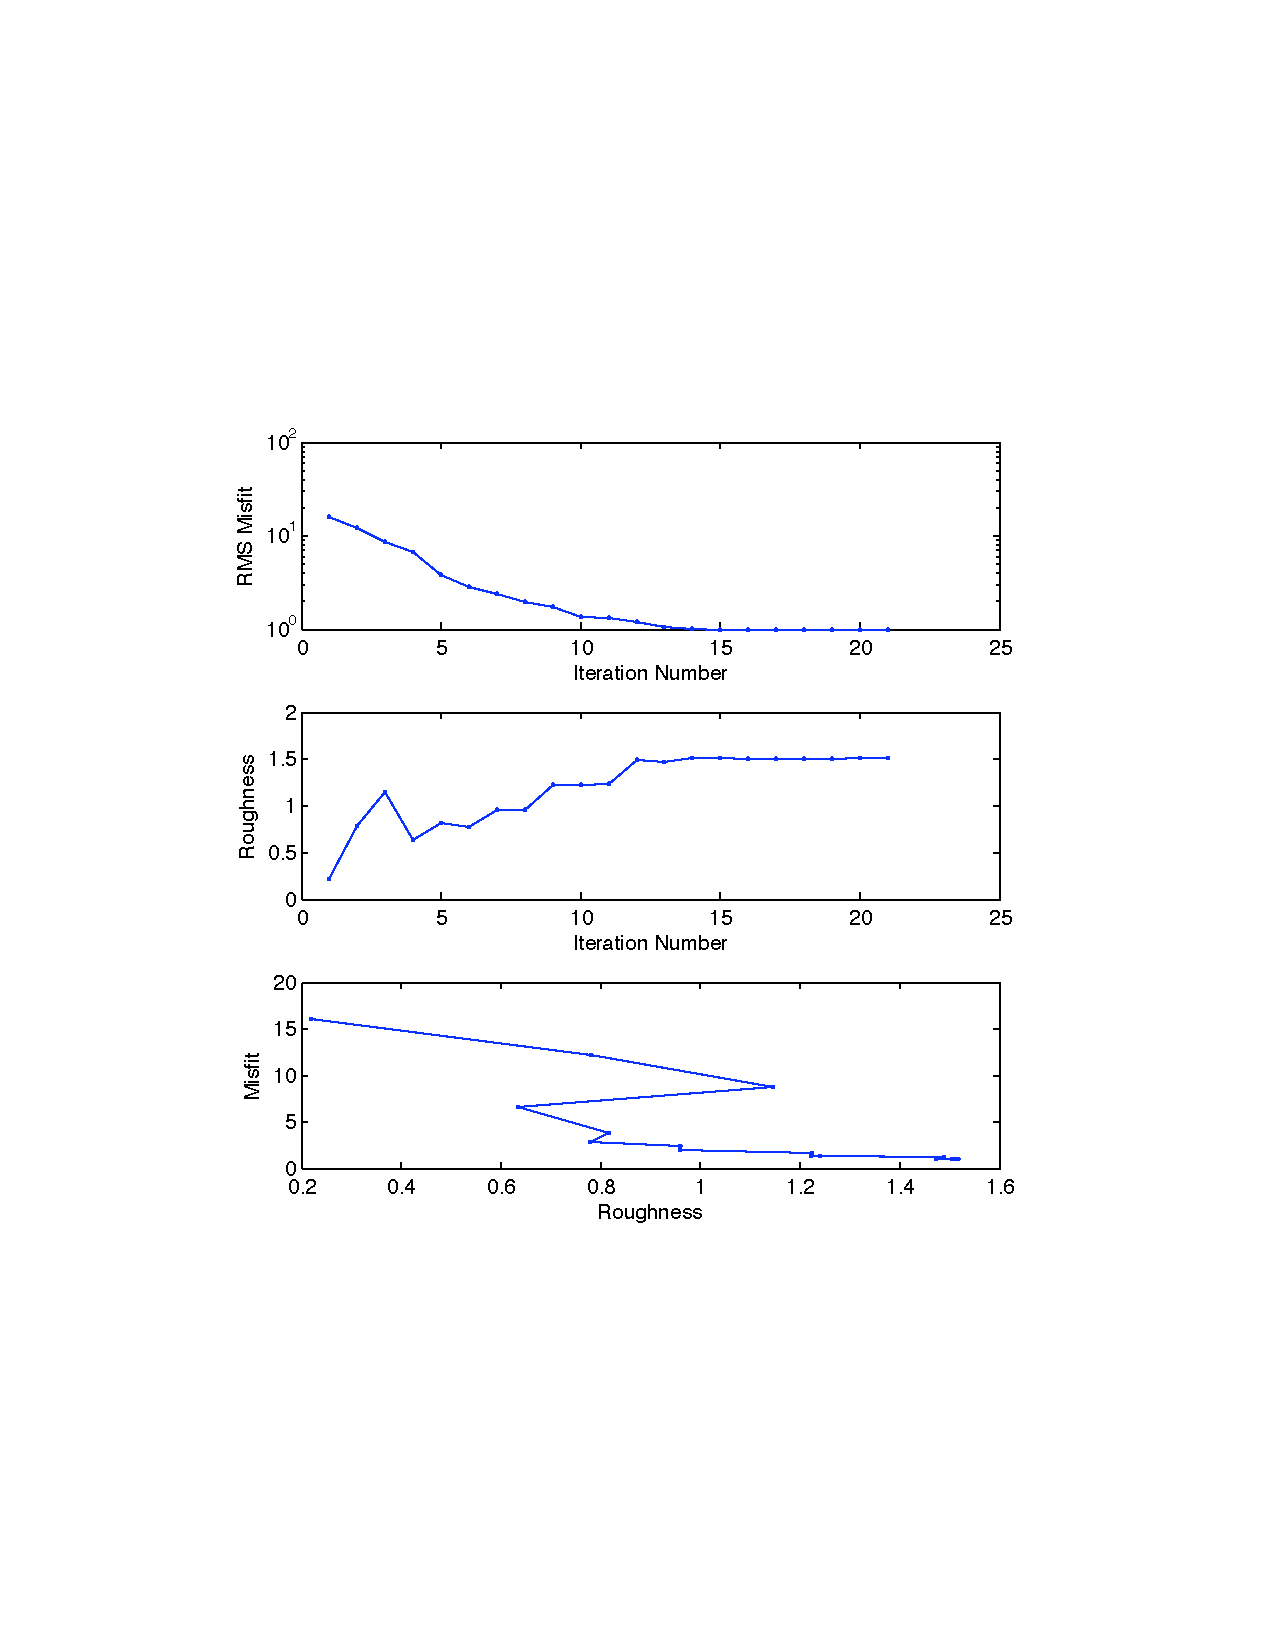
\includegraphics[width=.48\textwidth]{Figures/Misfit.pdf}
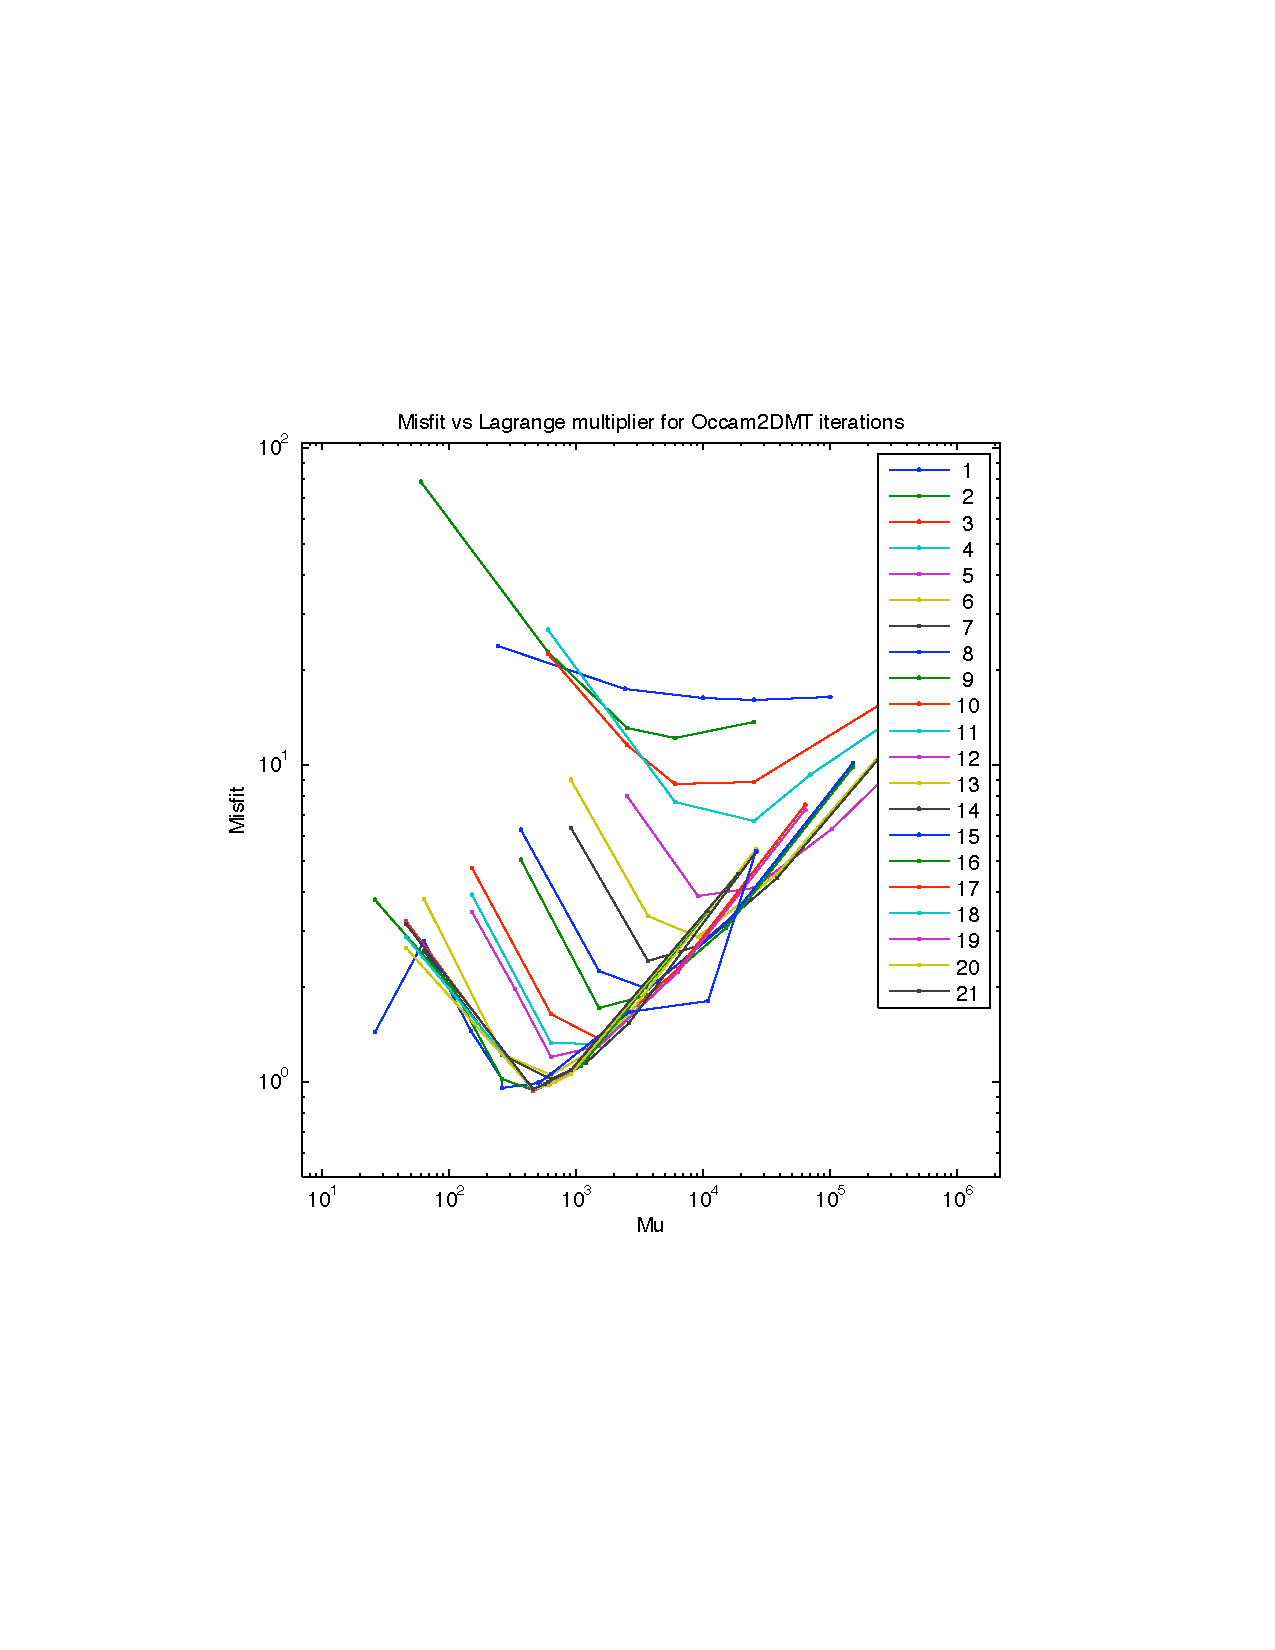
\includegraphics[width=.45\textwidth]{Figures/Mu.pdf}
\caption[plotOccam1DCSEMIterMisfit.m examples]{ plotOccam1DCSEMIterMisfit.m examples.  The left figure shows the RMS misfit and roughness versus iteration number, and versus each other. The right figure shows the misfit curve as a function of Lagrange multiplier $\mu$ for each inversion iteration (numbered in the legend). }
\label{fig:plotOccamIterMisfit}
\end{center}
\end{figure}
\clearpage



%-----------------------------------------------------------------------------------------------
\newpage
\subsection{Plotting data and model responses with plotCSEM.m }
%-----------------------------------------------------------------------------------------------
OCCAM1DCSEM comes with version 3.0 of the data plotting routine plotCSEM.m.  This routine originated with the MARE2DCSEM modeling code and has been updated here to handle plotting  survey data, model responses, data uncertainties and model fit residuals.
\\ \\
  Usage:
\begin{verbatim}
 >> plotCSEM       % creates an interactive menu for selecting data and
                   % plotting options. The rest should be obvious.
\end{verbatim}
        
 The interactive plotting menu used by plotCSEM.m is shown in Figure   \ref{fig:plotCSEMmenu}.   The following subsections describe the plotting options available with the various menus and buttons.              
                     
\begin{figure}[htbp]
\begin{center}
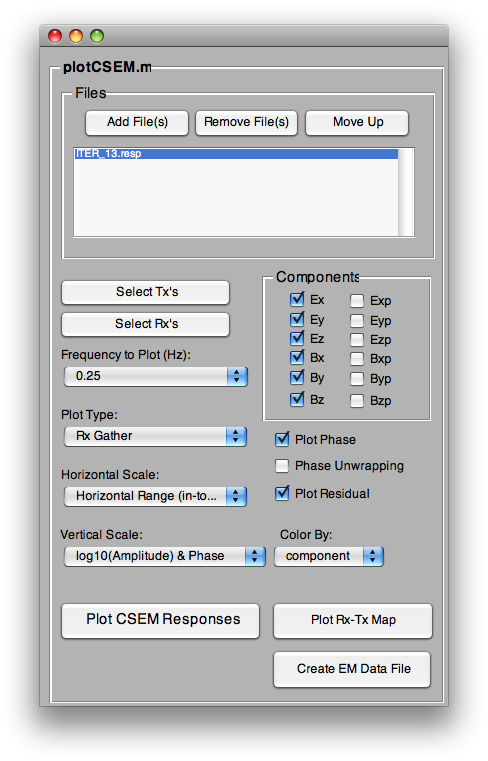
\includegraphics[width=.6\textwidth]{Figures/plotCSEM1}
\caption[plotCSEM.m menu figure]{ plotCSEM.m menu figure showing the plotting options available. }
\label{fig:plotCSEMmenu}
\end{center}
\end{figure}                    
                     \clearpage
                     
 
%-----------------------------------------------------------------
\subsubsection*{Add, Remove, Move Files}
%-----------------------------------------------------------------
In this section you can add .csem, .resp and .data files for plotting.  plotCSEM currently supports reading these data formats:
\begin{table}[htdp]
\begin{center}
\begin{tabular}{lp{4in}}
EMData\_1.1,EMData\_1.2 & Occam1DCSEM data file format \\
EMResp\_1.1,EMResp\_1.2 & Occam1DCSEM  model response file format \\
Dipole1D\_1.0,Dipole1D\_1.1 & DIPOLE1D forward model response file format \\
MARE2DCSEM\_2.0 & MARE2DCSEM finite element forward modeling code response file format. 
\end{tabular}
\end{center}
\label{tab:plotCSEMformats}
\end{table}
  
%-----------------------------------------------------------------
\subsubsection*{Frequency to Plot}
%-----------------------------------------------------------------  
Once you have some files added, this popup menu allows you to select the frequency to plot.

 %-----------------------------------------------------------------
\subsubsection*{Components}
%-----------------------------------------------------------------  
Check the boxes for the components to plot (if they are available in the data files).  The components ending with p, such as Eyp, are the primary fields computed for MARE2DCSEM models and aren't used for OCCAM1DCSEM plotting.  

 %-----------------------------------------------------------------
\subsubsection*{Select Tx's, Select Rx's}
%-----------------------------------------------------------------  
These buttons launch  listboxes that allows you to select which transmitters and receivers to plot, such as shown in Figure  \ref{fig:TxSelect}.  This is mainly used for only plotting subsets of Tx's and Rx's computed using MARE2DCSEM.

 \begin{figure}[htbp]
\begin{center}
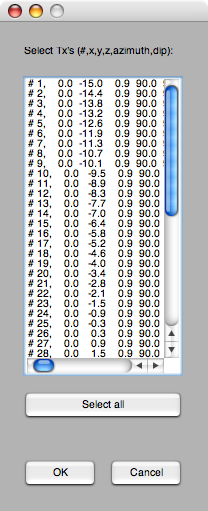
\includegraphics[width=.25\textwidth]{Figures/TxSelect.png} 
\caption{Transmitter selection list dialog.}
\label{fig:TxSelect}
\end{center}
\end{figure}
\clearpage
%-----------------------------------------------------------------
\subsubsection*{Plot Type}
%-----------------------------------------------------------------  
There are three plotting types:
\begin{itemize}
\item Tx Gather:  Data from each transmitter is plotted  at the position of each receiver.

\item Rx Gather: Data for each receiver is plotted  at the position of each transmitter.  This is what survey data recorded on a receiver are and hence is the type of plot commonly used with OCCAM1DCSEM modeling.  If the data file only contains a single receiver, then the plot type ``Rx Gather'' is automatically selected.
 \begin{figure}[h]
\begin{center}
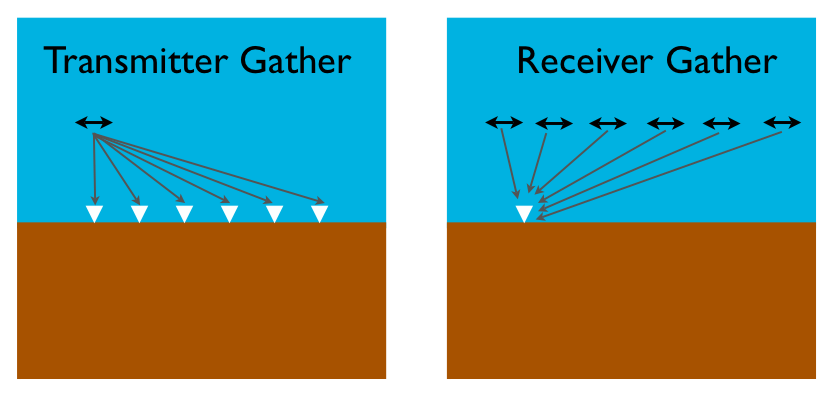
\includegraphics[width=.75\textwidth]{Figures/Gathers.png} 
\caption{Transmitter and receiver gathers.}
\label{fig:Gathers}
\end{center}
\end{figure}

\item Pseudosections:  Data from many transmitters and receivers are plotted at the source-reciever mid-point for the horizontal scale, and the signed source-receiver offset for the vertical scale.  This  currently only works for plotting MARE2DCSEM model responses.
 \begin{figure}[h]
\begin{center}
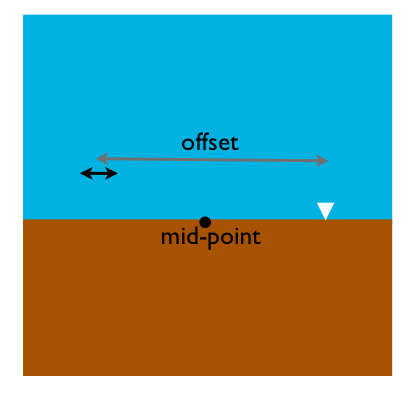
\includegraphics[width=.33\textwidth]{Figures/MidPointOffset.png} 
\caption{Mid-point and offset for pseudosection plots.}
\label{fig:Midpoints}
\end{center}
\end{figure}

\end{itemize}
\clearpage

 %-----------------------------------------------------------------
\subsubsection*{Horizontal Scale}
%-----------------------------------------------------------------  
Select the scale to use for the horizontal plotting axis. Choose from x, y, z,  Range (x,y,z), Horizontal Range (x,y), Horizontal Range (signed as InTow, OutTow),  Vertical Range and Rx-Tx Azimuth (useful for circular tows for anisotropy).


%-----------------------------------------------------------------
\subsubsection*{Vertical Scale}
%-----------------------------------------------------------------  
Set the vertical plotting scale.  Choose from
\begin{itemize}
\item log10 Amplitude and Phase.  
\item Real/Imaginary.  
\item Polarization Min/Max (horizontal only for now...)
\item Ratio: 2D/primary.  Only for MARE2DCSEM: Note that the primary response corresponds to the 1D primary model given in the RUNFILE. 
\item Relative Difference: (2D-primary)/primary. Only for MARE2DCSEM.
\end{itemize}
If two files have been added to the file list then you can create anomaly plot comparisons using these two options:
\begin{itemize}
\item Ratio: File 1 / File 2.   Only for MARE2DCSEM.
\item Relative Difference: (File 1-File 2)/File 2. Only for MARE2DCSEM.
\end{itemize}

%-----------------------------------------------------------------
\subsubsection*{Plot Phase}
%-----------------------------------------------------------------  
Checkbox for plotting phase (in addition to amplitude).

%-----------------------------------------------------------------
\subsubsection*{Phase Unwrapping}
%-----------------------------------------------------------------  
Checkbox for performing phase unwrapping.  Large phase jumps will be unwrapped so that phases can extend outside the $\pm 180^{\circ}$ window. This mostly  works, but can sometimes produce the wrong result for sparsely sampled or noisy data.

%-----------------------------------------------------------------
\subsubsection*{Plot Residual}
%-----------------------------------------------------------------  
Checkbox for selecting to plot the model response residuals (see equation \ref{eq:residual}) for OCCAM1DCSEM inversions.

%-----------------------------------------------------------------
\subsubsection*{Color By}
%-----------------------------------------------------------------  
Checkbox for selecting whether the data and model responses are colored by field component or file number.  It is useful to color by file if you want to compare the data fits for various OCCAM1DCSEM iteration response files.  If you're only plotting a single response file but which has many field components (for example $B_{x}, E_{y}$ and $E_{z}$), then it is useful to color by component.

%-----------------------------------------------------------------
\subsubsection*{Plot CSEM Responses}
%-----------------------------------------------------------------  
Once you've selected all the other plotting options, hit this button to create the plot.

%-----------------------------------------------------------------
\subsubsection*{Plot Rx-Tx Map}
%-----------------------------------------------------------------  
Hit this button to make a simple map plot showing the receiver and transmitter locations. The transmitters are plotted as short lines at the azimuth angles given in the data or response files.   This can be useful for verifying that the transmitter and receiver geometry in the data file is correct.

%-----------------------------------------------------------------
\subsubsection*{Create EM Data File}
%-----------------------------------------------------------------  
Hit this button to launch the createEMDataFile.m user interface.

%-----------------------------------------------------------------
\newpage
\subsection{Example Data and Response Plots}
%-----------------------------------------------------------------  

\begin{figure}[h]
\begin{center}
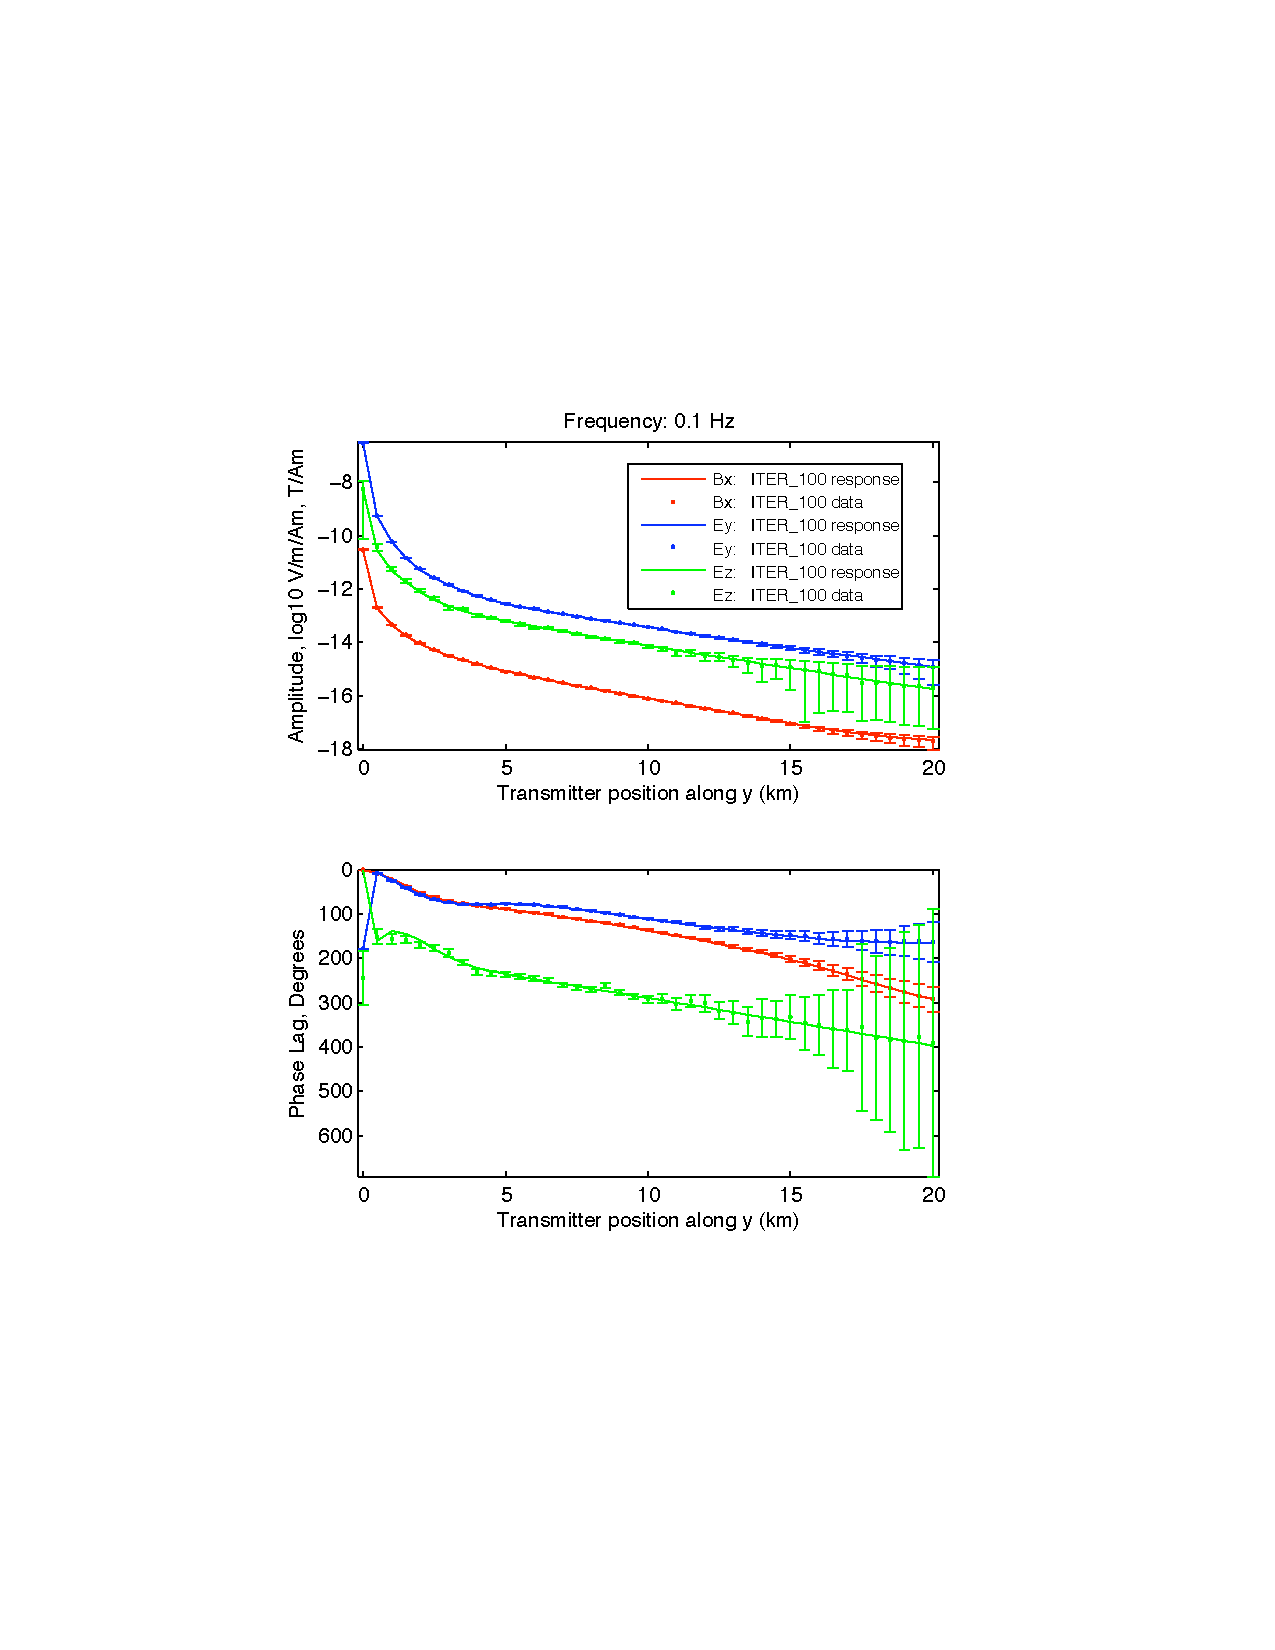
\includegraphics[width=.75\textwidth]{Figures/AmpPhs.pdf} 
\caption[Example amplitude and phase plot]{ Example amplitude and phase plot made with plotCSEM.m.  Data are plotted as dots with error bars and the model response for file ITER\_100.iter is shown as lines.}
\label{fig:AmpPhs}
\end{center}
\end{figure}           
                    
\begin{figure}[h]
\begin{center}
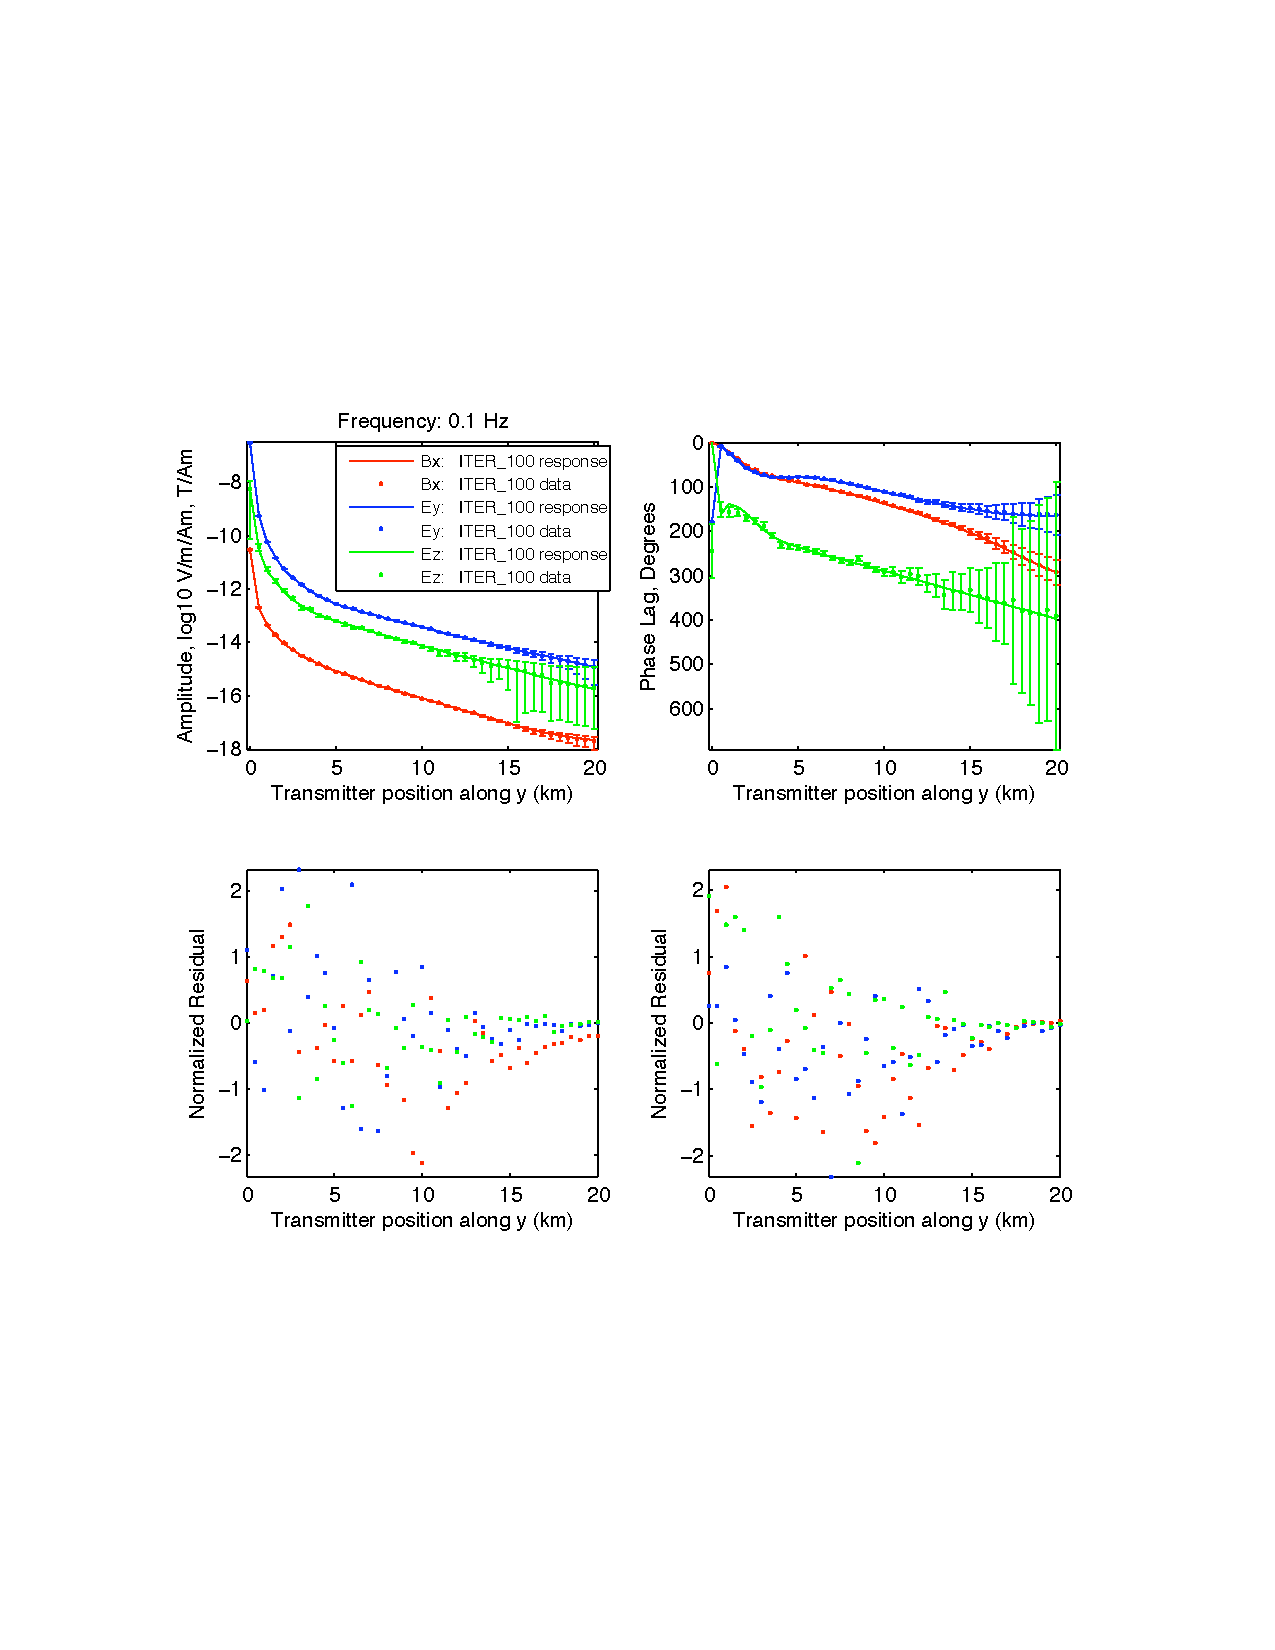
\includegraphics[width=.9\textwidth]{Figures/AmpPhsResid.pdf} 
\caption[Example amplitude and phase plot with residuals]{ Example amplitude and phase plot with residuals, made with plotCSEM.m.  The lower row  shows the amplitude residual (left) and phase residual (right). A good fit to the data will have residuals that are largely uncorrelated.  }
\label{fig:AmpPhsResid}
\end{center}
\end{figure}                 
 
 \begin{figure}[h]
\begin{center}
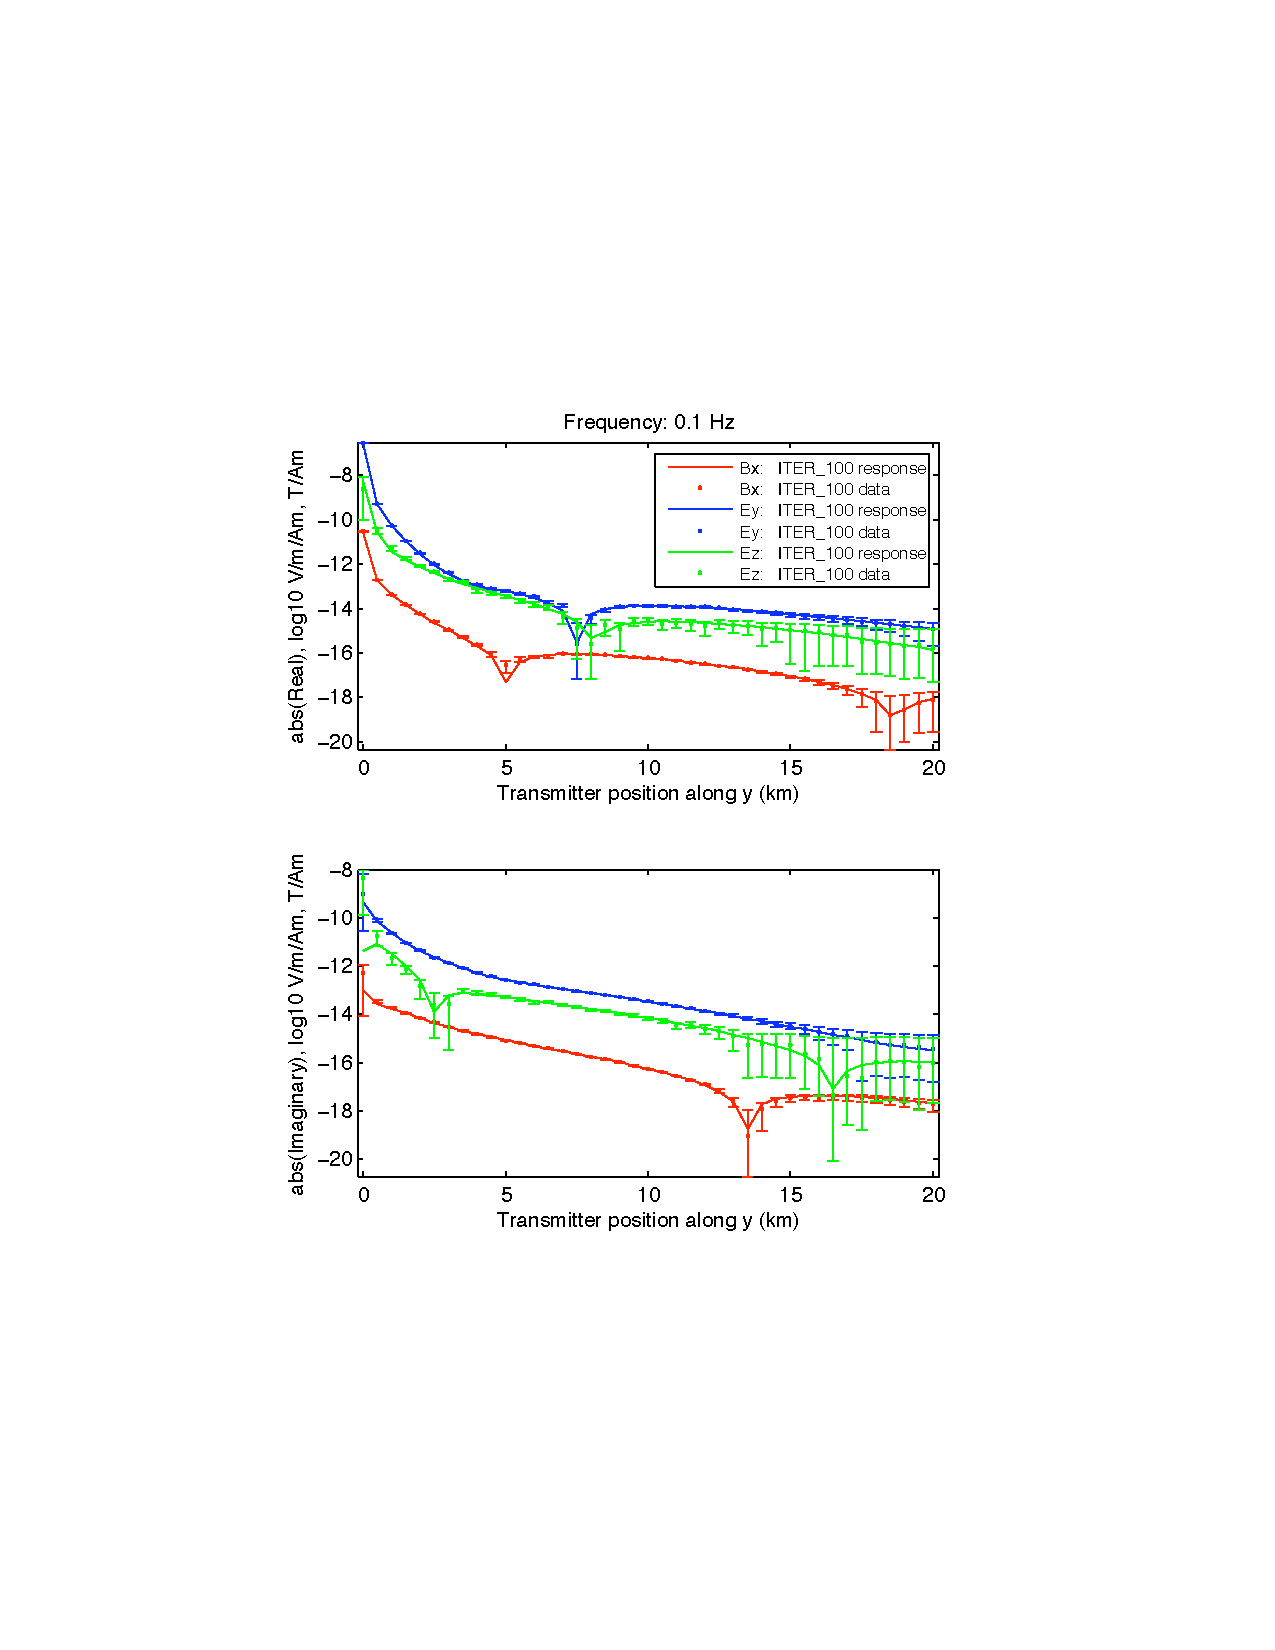
\includegraphics[width=.7\textwidth]{Figures/RealImag.pdf} 
\caption[Example real and imaginary plot]{Example real and imaginary plot made with plotCSEM.m.  The valleys in the responses are where the components have a zero crossing.   Zero crossings in the real component denote where the phase crosses an odd integer multiple of $90^{\circ}$. Zero crossings in the imaginary component denote where the phase crosses an integer multiple of $180^{\circ}$.}
\label{fig:RealImag}
\end{center}
\end{figure}   
  
  \begin{figure}[h]
\begin{center}
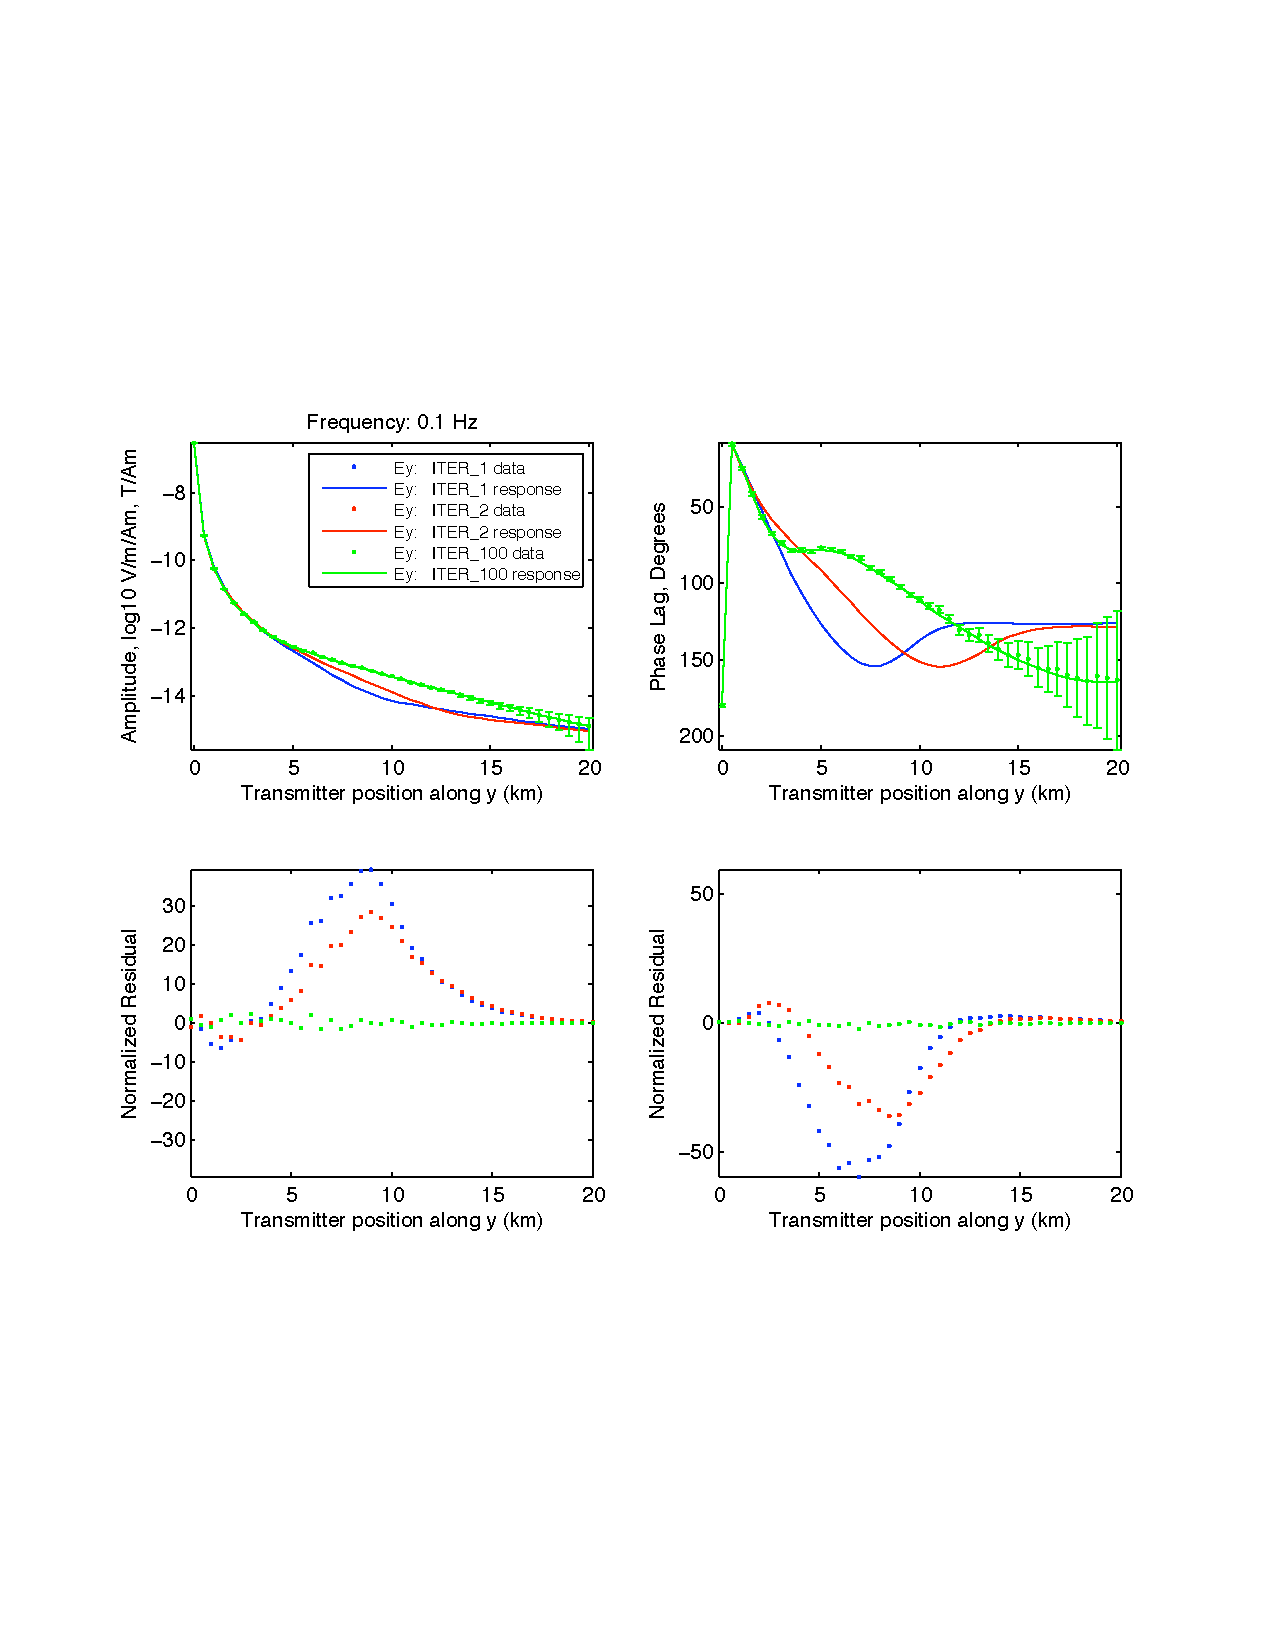
\includegraphics[width=.9\textwidth]{Figures/ColorByFile.pdf}
\caption[Example of coloring plots by file]{Example of coloring plots by file in plotCSEM.m. The three colors show the $E_{y}$ responses for iterations 1, 2 and 100. Note the difference in the residual plots (iteration 100 fits to RMS 1.0).  }
\label{fig:ColorByFile}
\end{center}
\end{figure}    


    
                                    
 
%-----------------------------------------------------------------------------------------------
\clearpage
\section{OCCAM1DCSEM Examples}
%-----------------------------------------------------------------------------------------------
This section presents a few figures demonstrating results from the new OCCAM1DCSEM inversion.  Some of these examples are present in the /Examples folder.


\subsection{San Diego Trough CSEM Data}
\begin{figure}[h]
\begin{center}
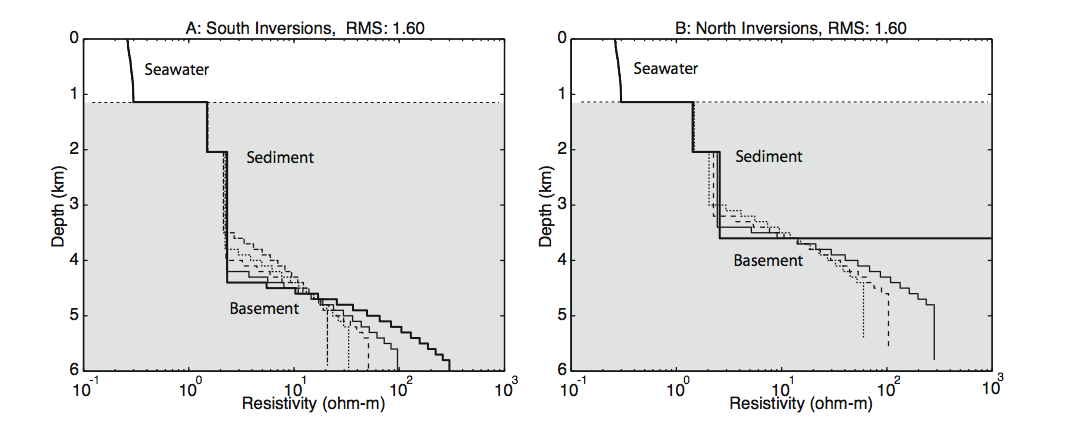
\includegraphics[width=\textwidth]{./Figures/Trough}
\caption[San Diego Trough data inversions]{OCCAM1DCSEM inversion of CSEM survey data collected in the San Diego Trough for tows to the south (left) and north (right) of a long-wire EM receiver.  The inversions included the stratified seawater resistivity as fixed structure and the shallow sediments where divided into two free layers based on seismic and gravity studies, and these were underlain by many thin layers for the basement.  In order to study the sensitivity to the depth of the resistive basement, the  thickness of the second sediment layer was varied between inversions (shown by the various lines). From \citet{SDTrough}.  The data used in these inversions are available in /Examples/SanDiegoTrough.}
\label{fig:Trough}
\end{center}
\end{figure}

\clearpage
\subsection{Component Resolution Tests on Synthetic Data}
\begin{figure}[h]
\begin{center}
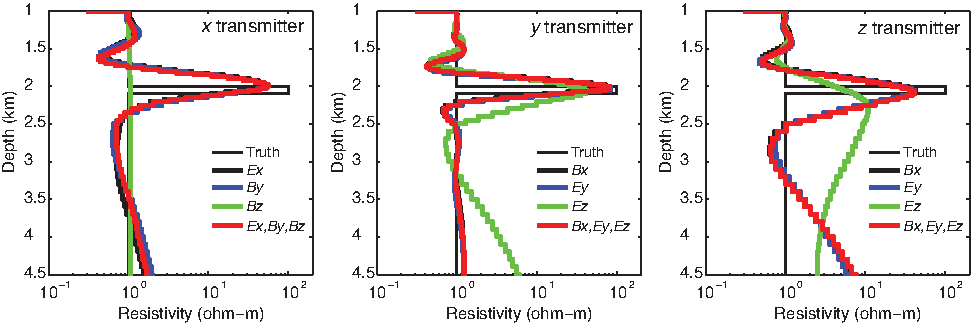
\includegraphics[width=\textwidth]{./Figures/ComponentInversion}
\caption[Synthetic component inversion resolution tests]{The resolution of the {\bf E} and {\bf B} field components for the three fundamental transmitter orientations (broadside x, inline y, and vertical z) for a line of receivers along the $y$ axis. Synthetic inversion models are shown for inversion of each component separately and all three together, as indicated in the legends.  The transmission frequencies were 0.1 and 1.0 Hz, the data had 1\% noise added and all models fit the data to  RMS 1.0. From \citet{key:F9}.}
\label{fig:ComponentInversion}
\end{center}
\end{figure}

\clearpage
\subsection{Synthetic  Data from Thinly Layered Sediments: Smooth and  Penalty Cut  Inversions }
\begin{figure}[h]
\begin{center}
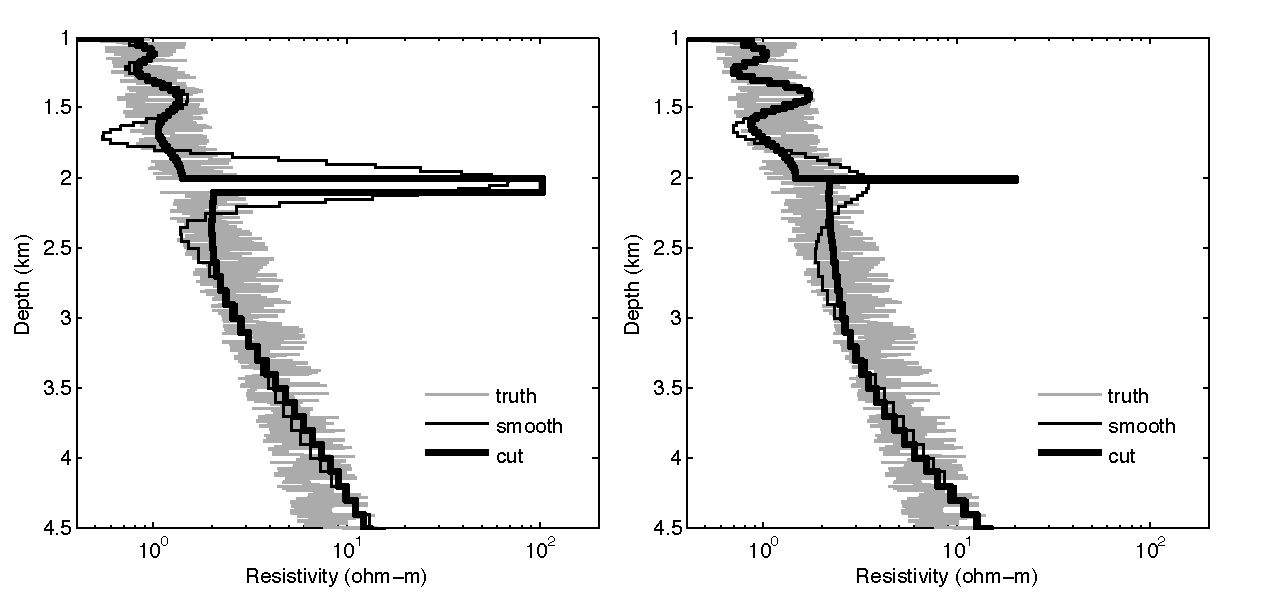
\includegraphics[width=\textwidth]{./Figures/aniso}
\caption[Synthetic inversions from fine layered models]{OCCAM1DCSEM inversion of synthetic CSEM data computed for the finely layered models shown by the gray lines. Both smooth inversion (all penalty weights set to 1) and penalty cut inversions (penalty weights set to 0 on reservoir boundaries) are shown. From \citet{key:F9}.}
\label{fig:Aniso}
\end{center}
\end{figure}

\clearpage
\subsection{ Minimum Gradient Support Roughness Penalty Examples }
\begin{figure}[h]
\begin{center}
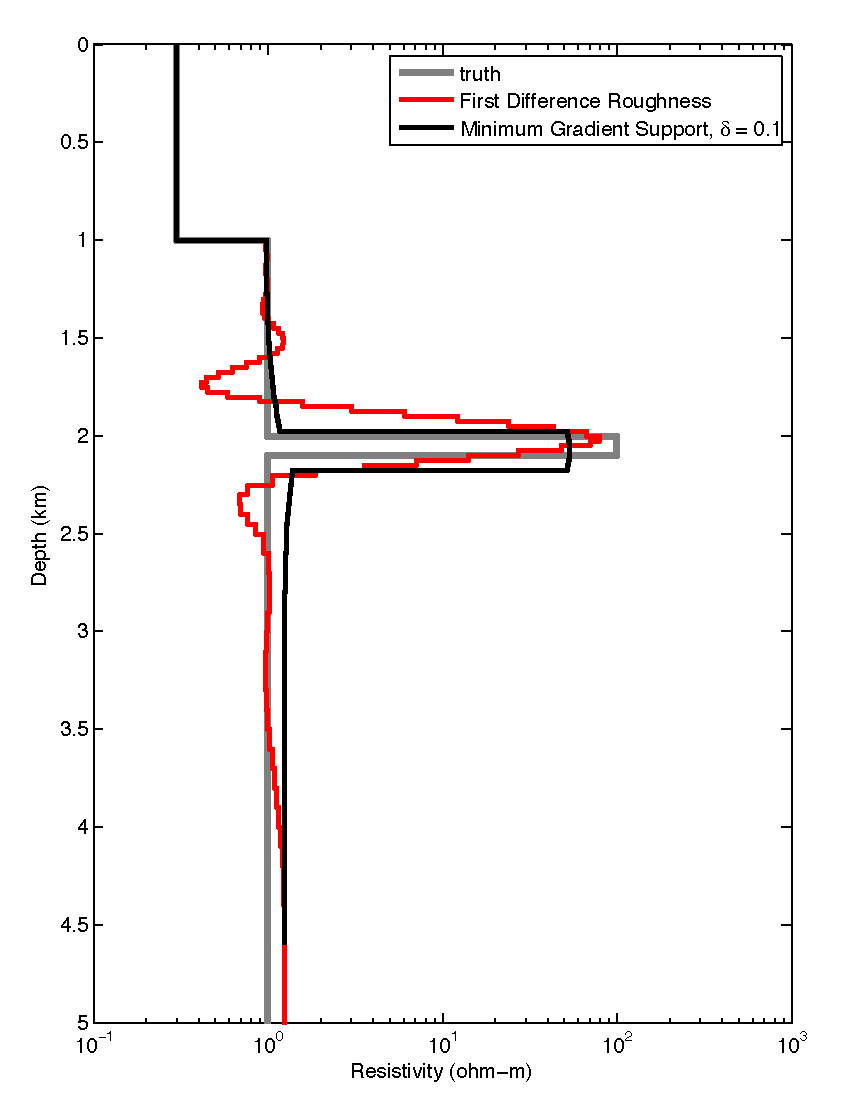
\includegraphics[width=3.2in]{Figures/Canonical_mgs.pdf}
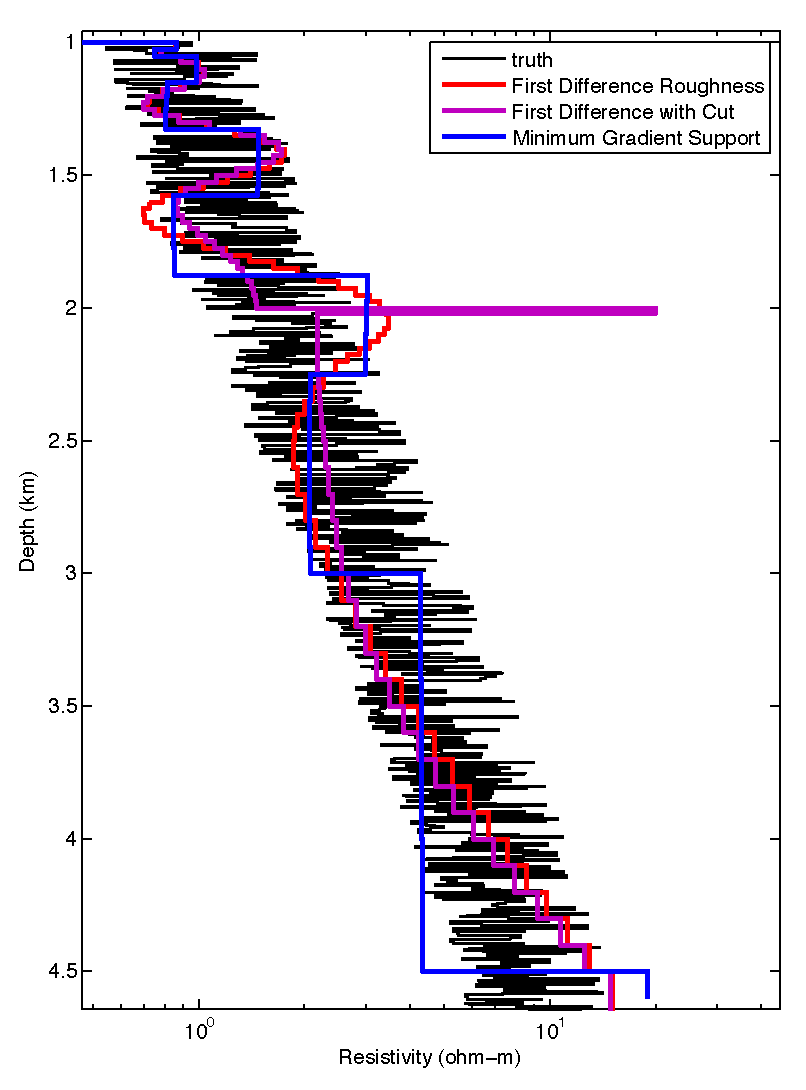
\includegraphics[width=3in]{Figures/Comparison_thin_mgs.pdf}
\caption[Minimum gradient support inversion examples ]{ Examples of inversion models obtained using minimum gradient support roughness penalty compared with inversions using standard first-difference roughness.  For the large resistive target in the canonical 1D model (left), both regularizations result in models that identify the presence of a large resistor, while the minimum gradient support  inversion produces a more geologically pleasing discrete resistive layer.  However, for much smaller targets such as the 10 m thick, 10 ohm-m reservoir in the model on the right, the minimum gradient support inversion is perhaps less pleasing than the smooth first difference model, while neither provides strong indication of the thin reservoir layer.  In these hard target cases, adding structural information via penalty cuts can help isolate small resistive layers. }
\label{fig:MGS}
\end{center}
\end{figure}


 
\clearpage
\subsection{Joint Inversion of CSEM and MT Data }
\begin{figure}[h]
\begin{center}
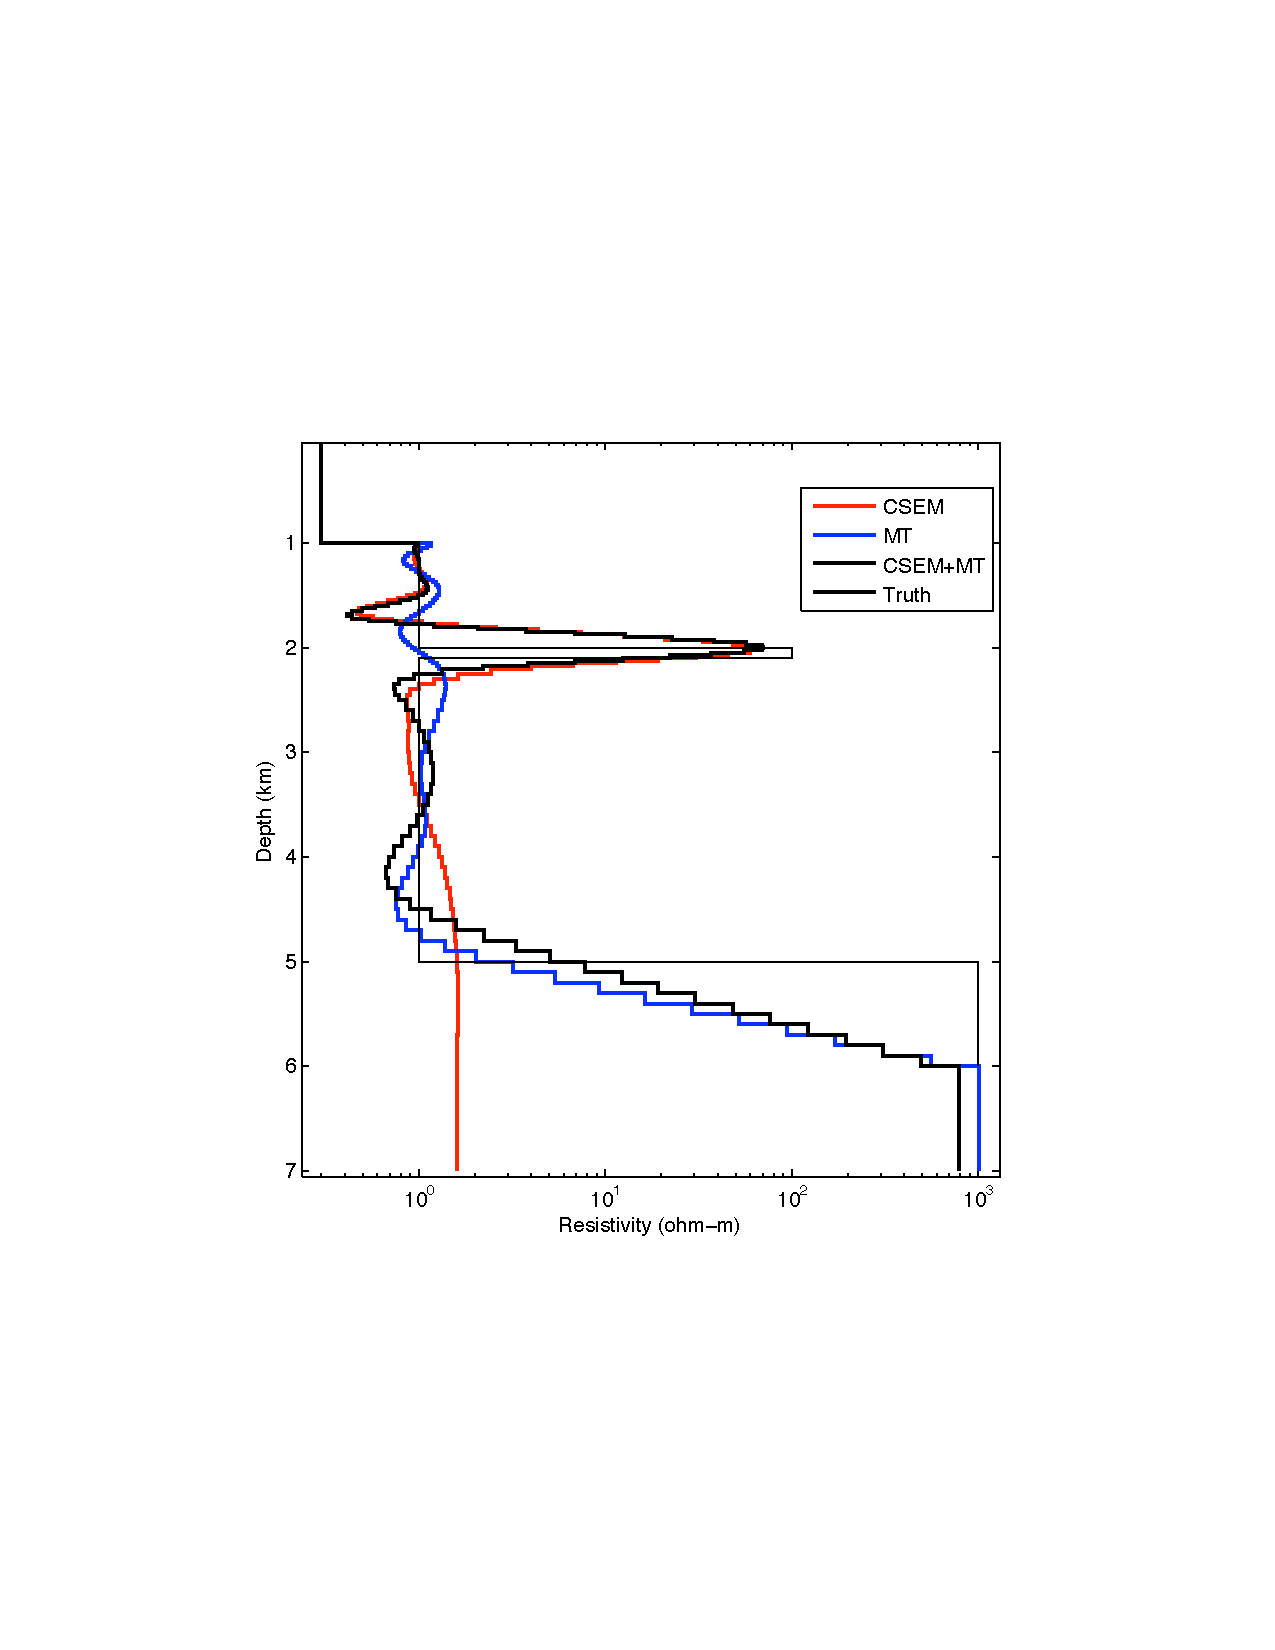
\includegraphics[width=.6\textwidth]{./Figures/CSEM_MT.pdf}
\caption[Joint Inversion of CSEM and MT Data]{ Synthetic inversions of CSEM and MT data inverted both independently and jointly, as indicated in the legend.  The synthetic CSEM data consisted of 0.1 and 1.0 Hz with 2\% noise added, while the MT data used 21 frequencies from 0.0001 to 1 Hz.  The CSEM data are sensitive to the sediments and reservoir while the MT data are sensitive to the sediments and basement.  The joint inversion is able to recover both the reservoir and the basement.  These models and data are available in /Examples/CanonicalBasement\_CSEM\_MT  }
\label{fig:Aniso}
\end{center}
\end{figure}
 
\clearpage
\subsection{Bounding  the Model Parameters During Inversion}
\begin{figure}[h] 
\begin{center}
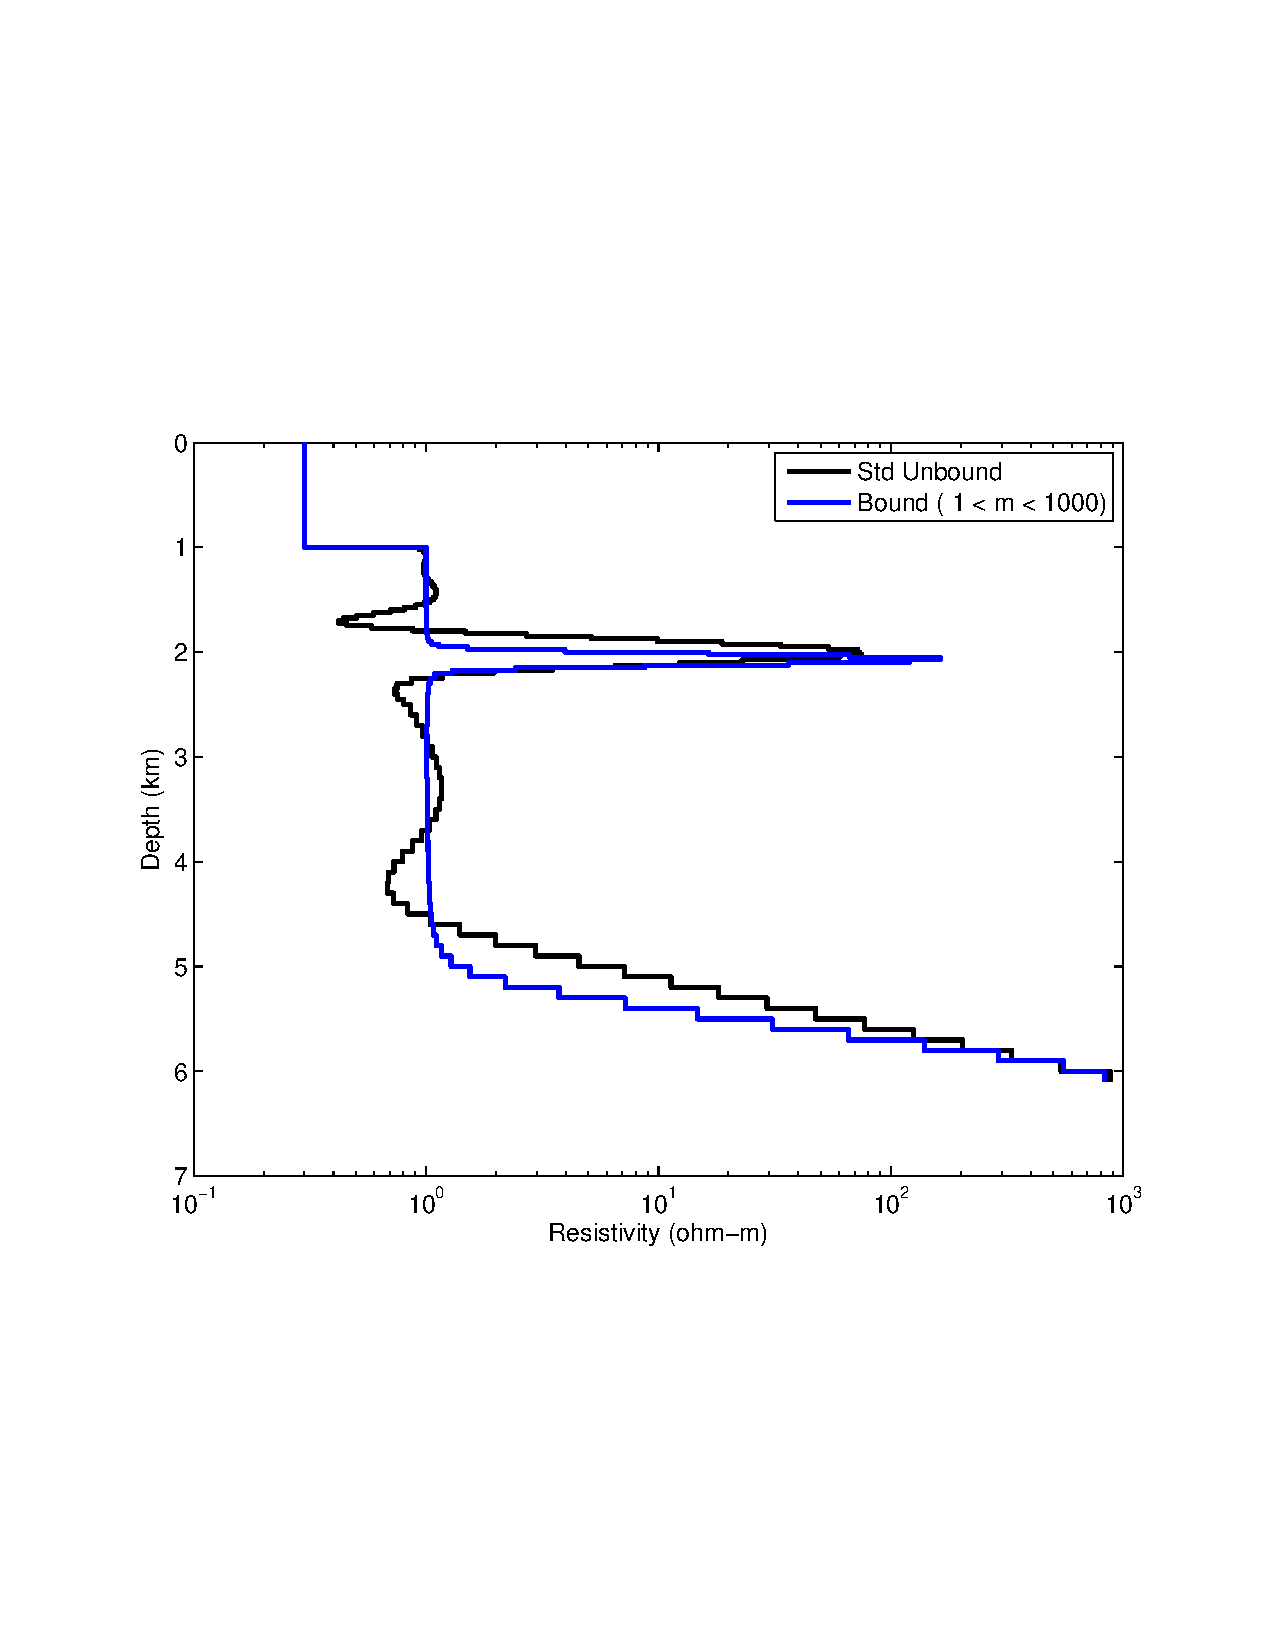
\includegraphics[width=.6\textwidth]{./Figures/BoundExample.pdf} 
\caption[Inversion using model bounds]{ Example of in inversion with bounds on the model parameters.  Here we use the same CSEM and MT synthetic data as for the last example, but now with bounds. Notice how the bound inversion is improved since it can no longer drop below 1 ohm-m.  You can find the files for this inversion test in the folder: /Examples/Synthetic/CanonicalPlusBasement/CSEM\_MT\_bound.  }
\label{fig:Bounds} 
\end{center}
\end{figure}  

\clearpage

%-----------------------------------------------------------------------------------------------
\section{Troubleshooting}
%-----------------------------------------------------------------------------------------------


%-----------------------------------------------------------------------------------------------
\subsection{I removed the roughness penalty on some of the layers and now it won't converge to a reasonable misfit.}
%-----------------------------------------------------------------------------------------------
Removing the roughness penalty can sometimes destabilize the inversion (hence the reason the roughness penalty is also called a stabilizer and is heavily relied upon for EM inversion).  If you find the inversion has trouble with this, try adding a preference resistivity value for the layers with the cut roughness penalty, and make sure you include a non-zero preference penalty value (try something in the range of 0.01 to 1).    You can also stabilize the inversion by setting values for the ``Model Limits'' field in the Occam startup file.   For example,``Model Limits:   -1,4'' will force the resistivity to stay between 0.1 and 10,000 ohm-m.  

%-----------------------------------------------------------------------------------------------
\subsection{My inversion model looks awful!} 
%-----------------------------------------------------------------------------------------------
Most likely this is a case of  ``garbage in = garbage out".  First check that you have the correct phase convention set for your data.  For example, compute the forward response for a likely model and check that phases
are either increasing or decreasing in accordance with the data. If not, use the opposite phase convention by specifying the convention in the data file (see section \ref{sec:Phase}).  The next thing to check is that you have the right receiver and transmitter geometries and rotations.  Finally, you should visually inspect the data to ensure that it is free of extended periods of  noise-floor level data. Also make sure that there are no strong outliers in the data.  For example, single data points ten times off the main trend can wreak havoc since it will contribute 100x to the L2 norm.  Search the Occam1DCSEM residuals in the .resp files for any large outliers. If you find some,  either remove the corresponding data or greatly increase its uncertainty level.  You may need to iterate on this for a few inversion runs. 


 
%-----------------------------------------------------------------------------------------------
\newpage
\bibliographystyle{seg}
\bibliography{embib}
%\bibliography{/Users/kkey/Documents/TEX/EMbib}

\end{document}  